\section{Equipment Module}\label{sec:01}

\subsection{Equipment Class}

In order to perform classification of equipment correctly, users can create equipment classes. Possible equipment classes are hose pipe, ladder, lamp, etc. When creating a new equipment class, users have to fill in its title without white spaces and activity status, as well as its description, as displayed on \hyperref[sections/equipment/images/Fig.1]{Fig.~\ref*{sections/equipment/images/Fig.1}}.

	\begin{figure}[!htbp]
	\centering
	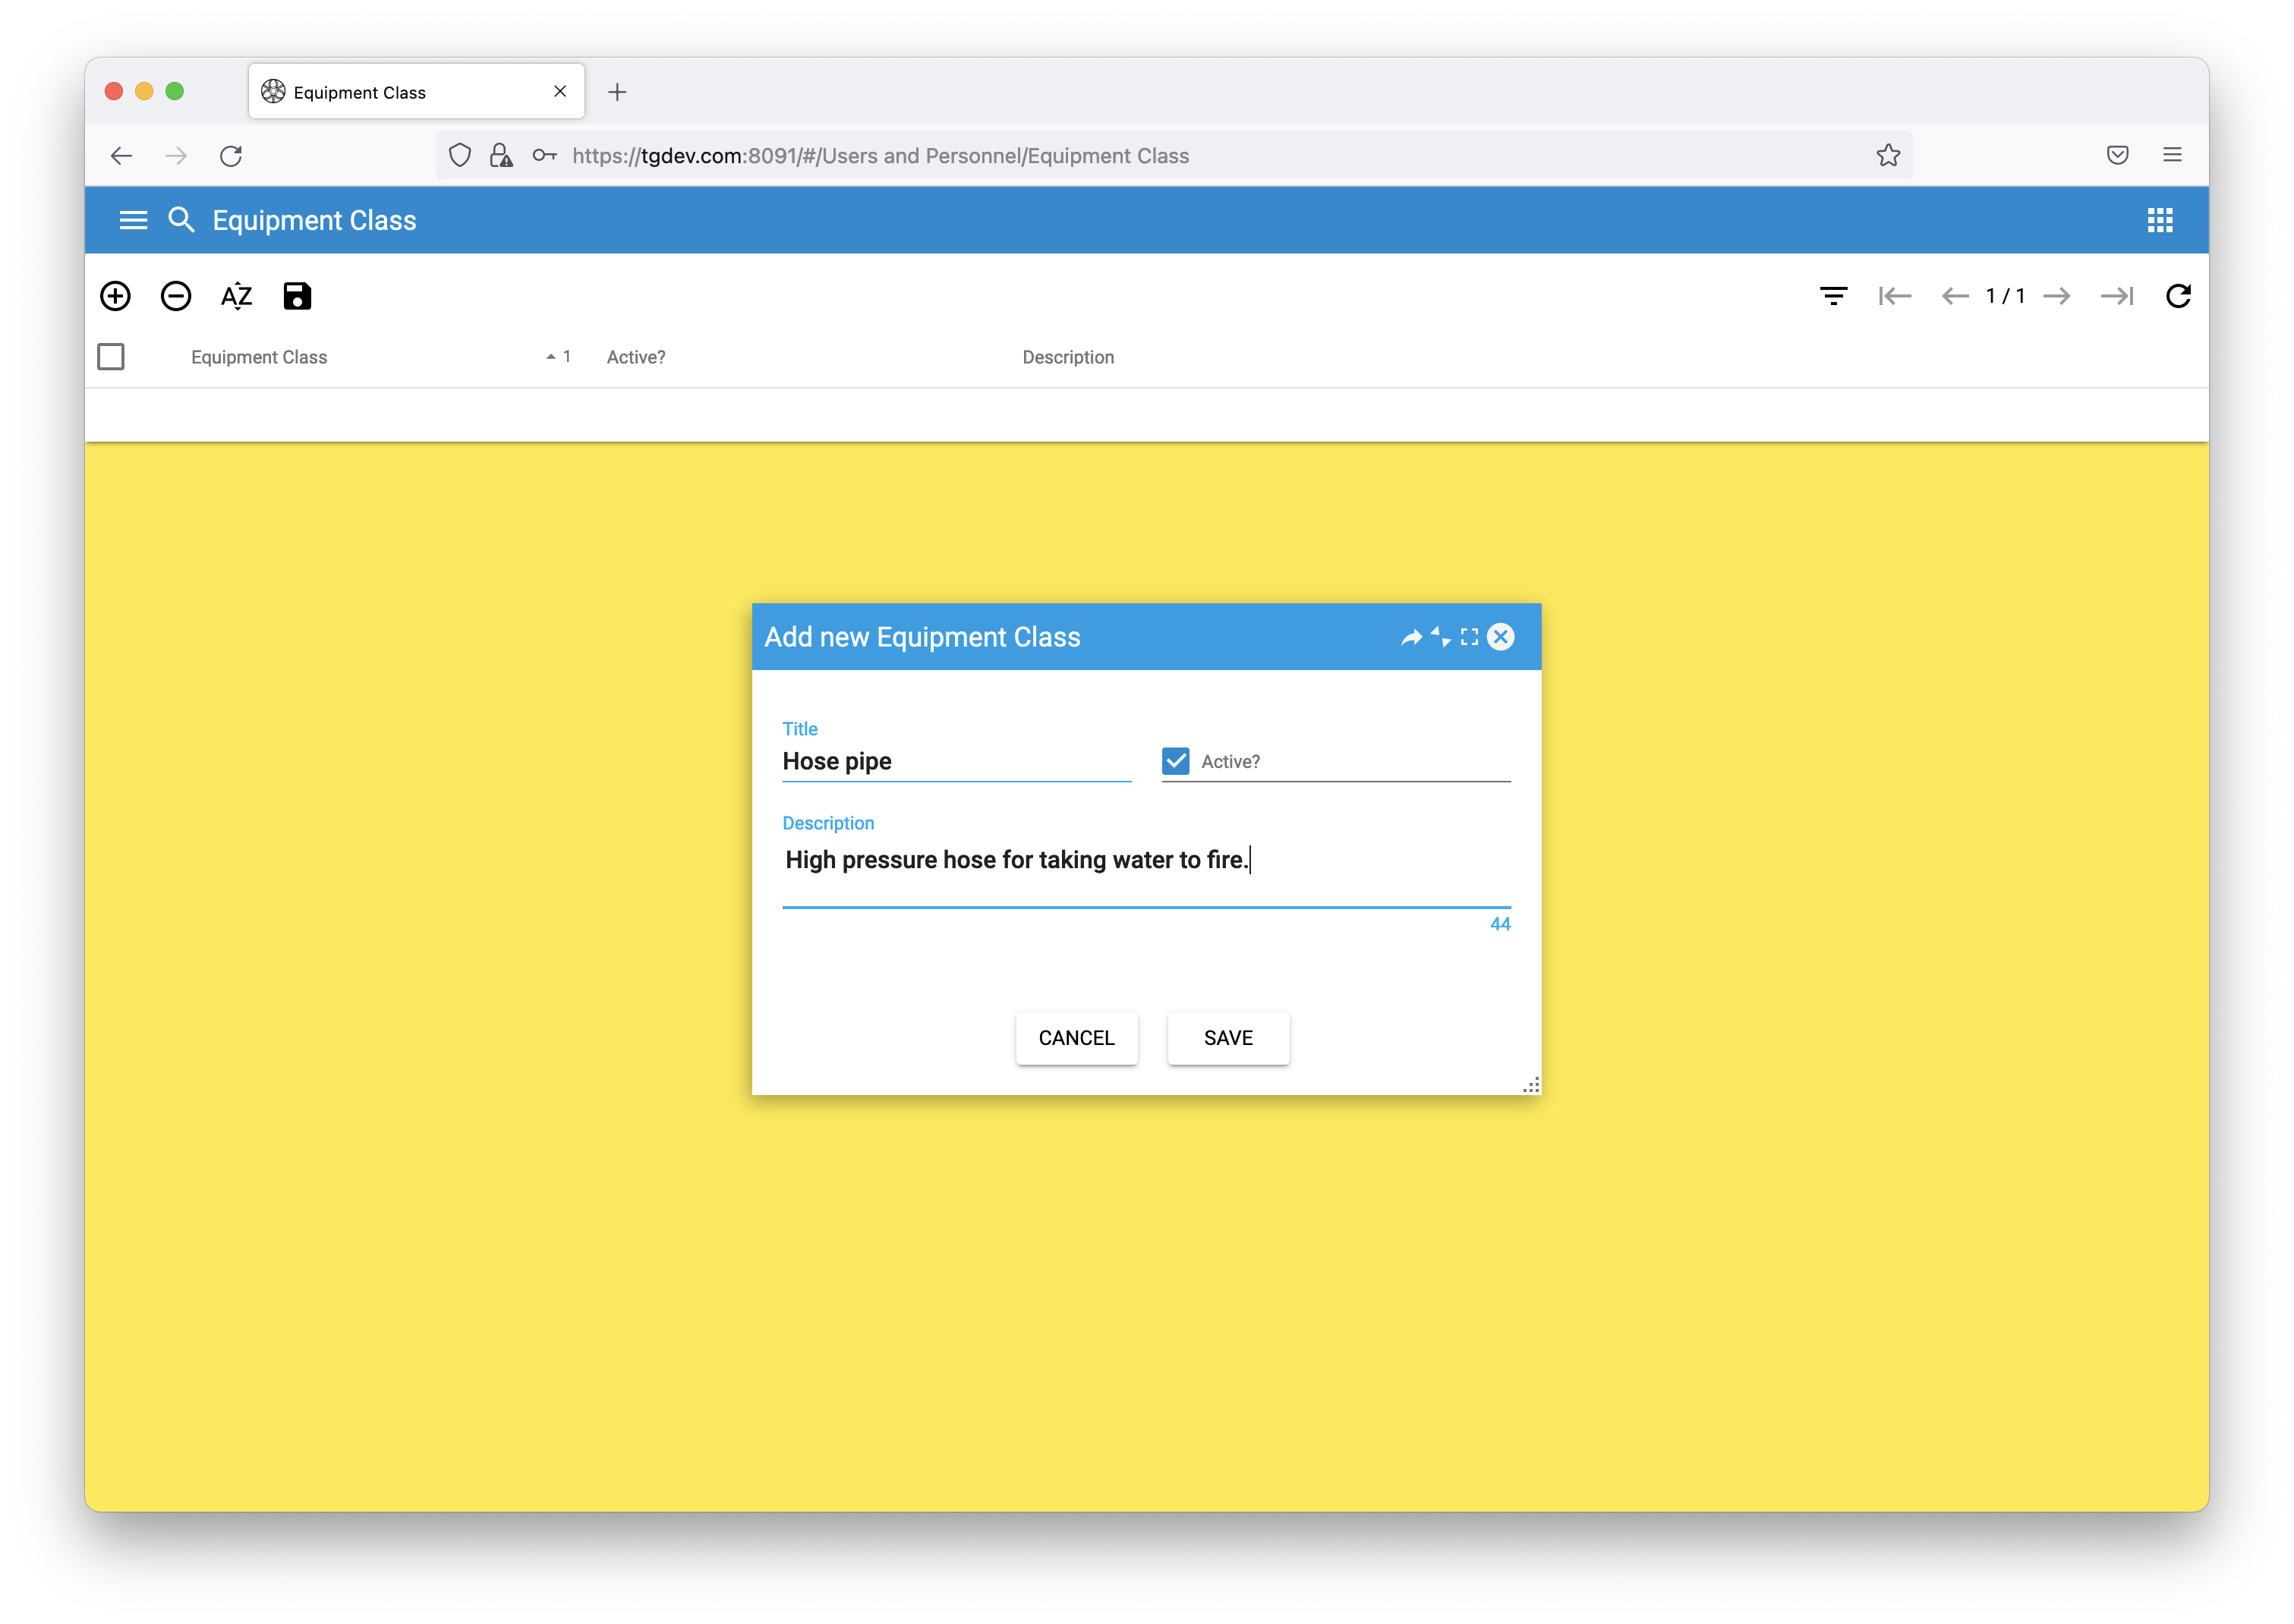
\includegraphics[width=0.95\linewidth]{sections/equipment/images/Fig.1.png}
	\caption{Equipment class creation.}\label{sections/equipment/images/Fig.1}
	\end{figure}
	
Users can search for existing equipment classes either by specifying title, which is auto-completed, or activity status, or both, as displayed on \hyperref[sections/equipment/images/Fig.2]{Fig.~\ref*{sections/equipment/images/Fig.2}}.

    \begin{figure}[!htbp]
	\centering
	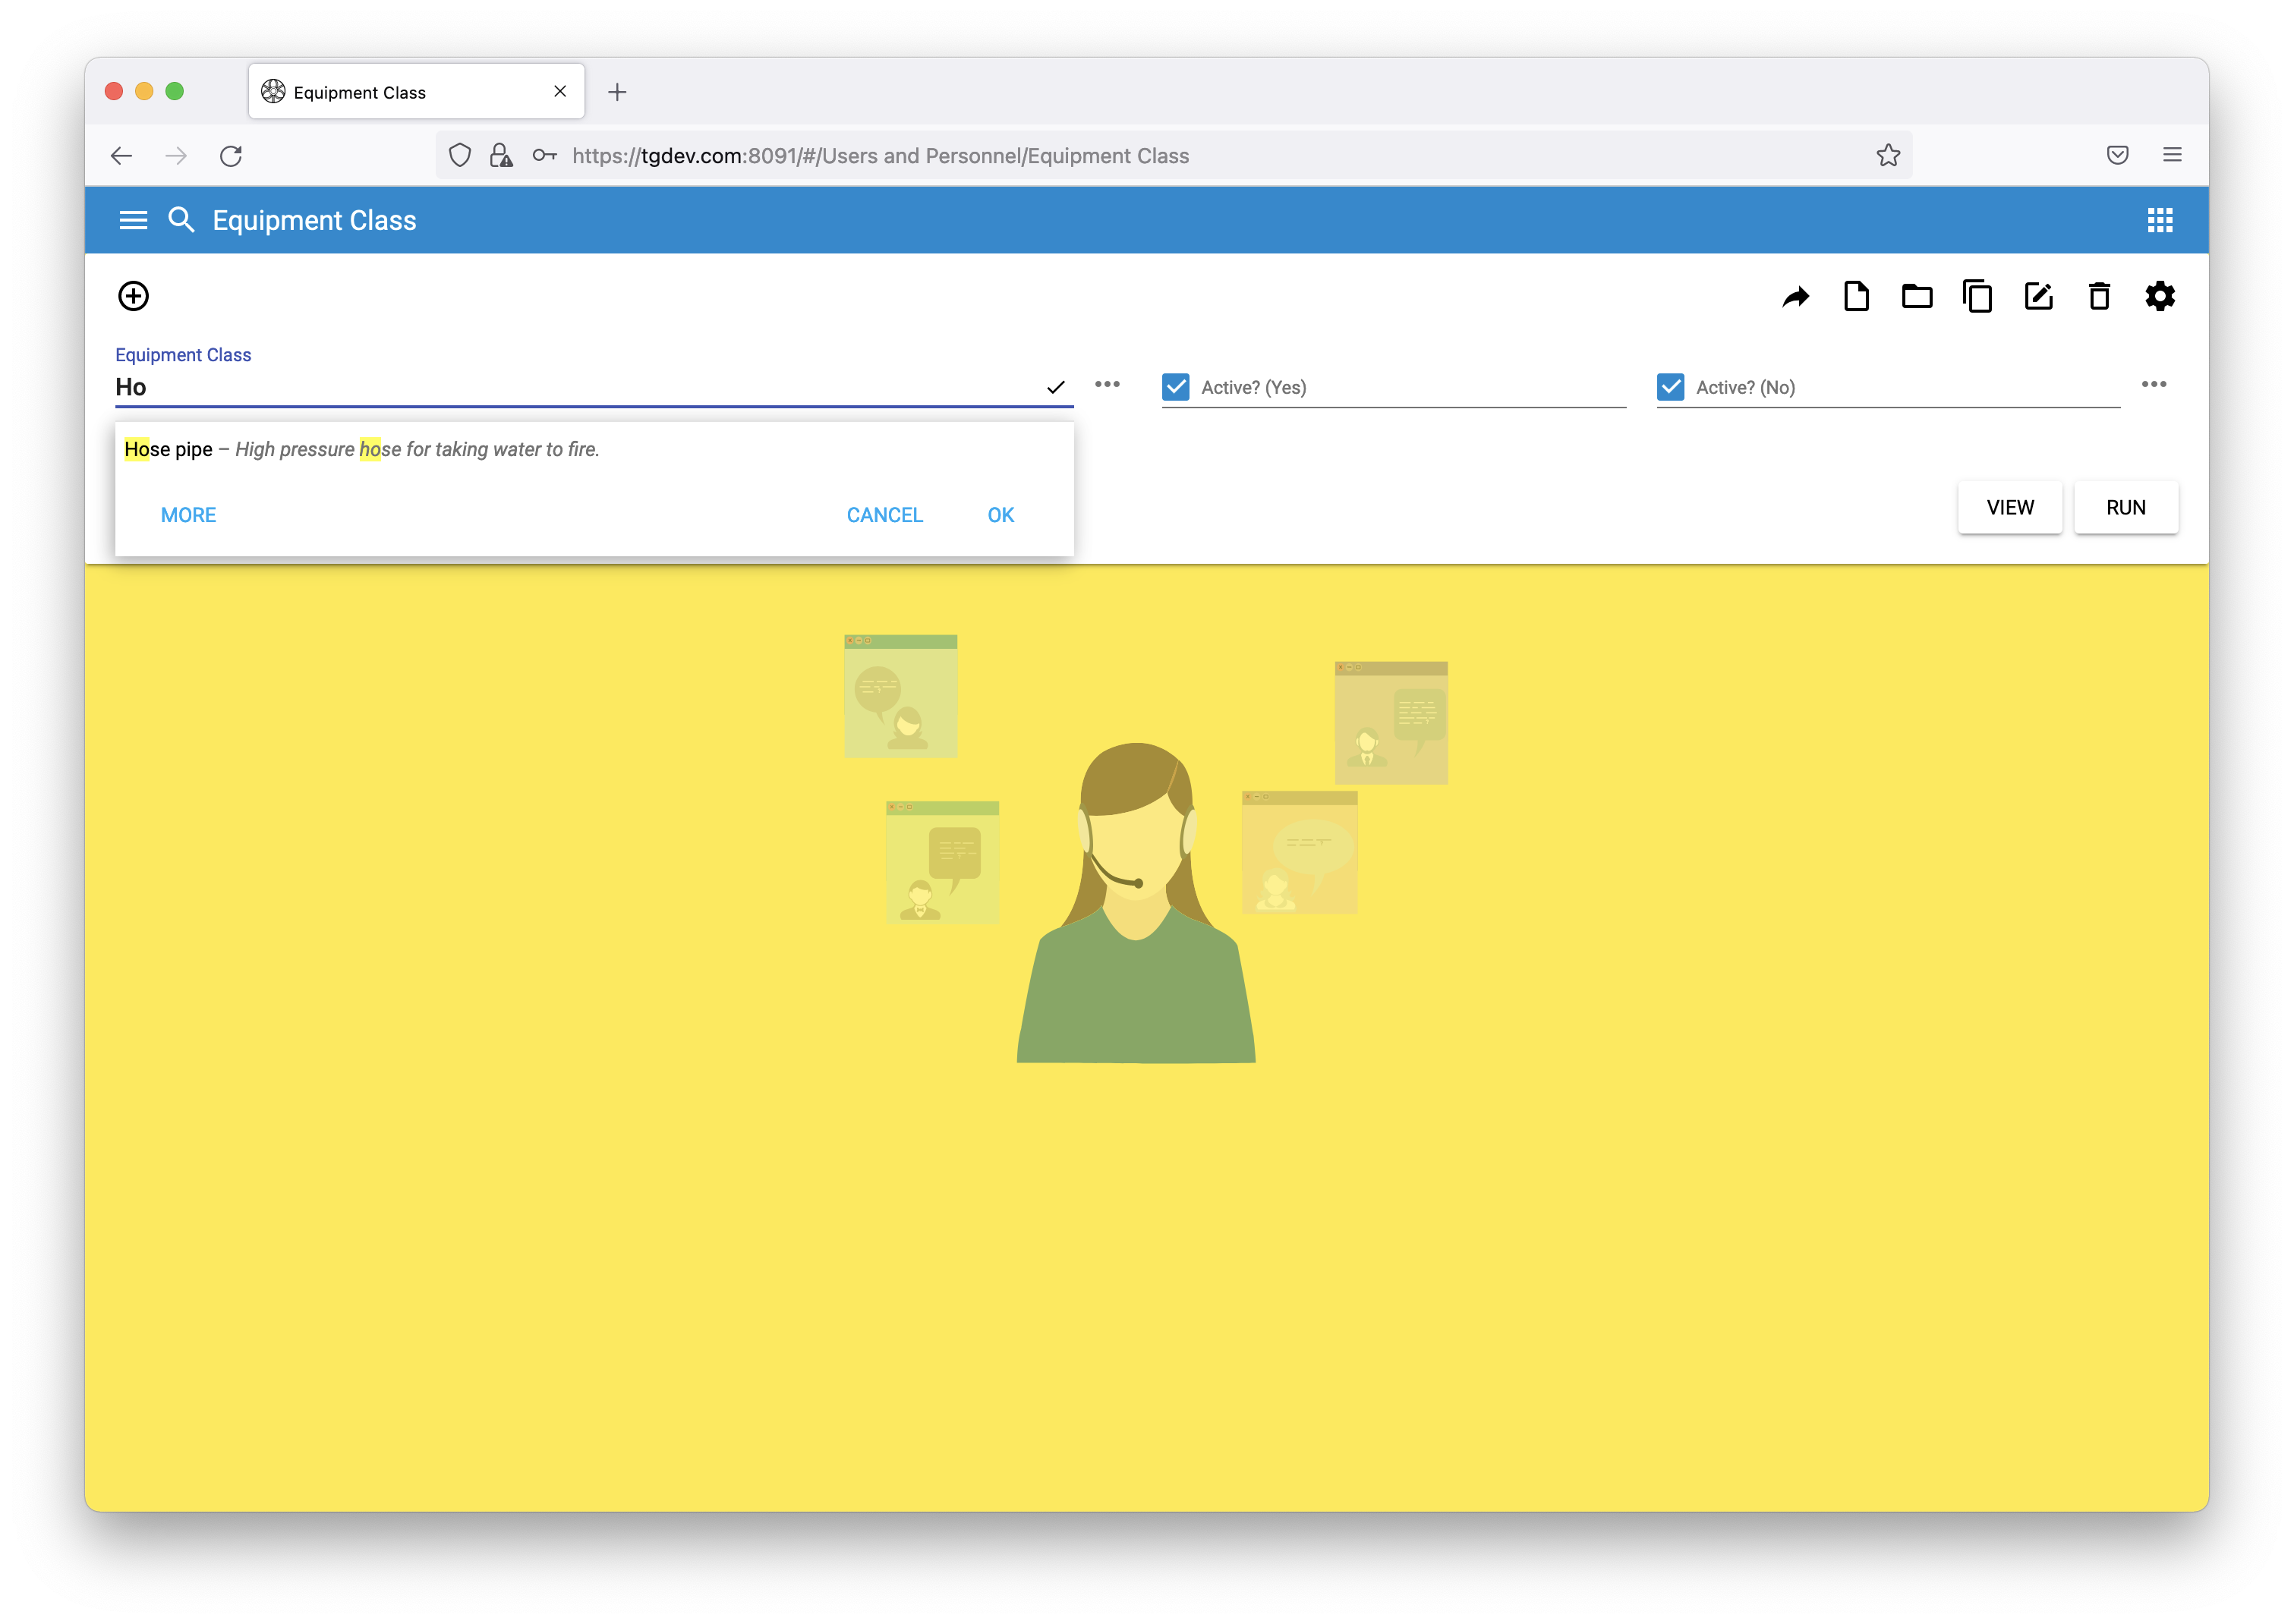
\includegraphics[width=0.95\linewidth]{sections/equipment/images/Fig.2.png}
	\caption{Equipment search query.}\label{sections/equipment/images/Fig.2}
	\end{figure}

\newpage
Search results are displayed along with title, activity status and description of the relevant equipment classes, as displayed on \hyperref[sections/equipment/images/Fig.3]{Fig.~\ref*{sections/equipment/images/Fig.3}}.

    \begin{figure}[!htbp]
	\centering
	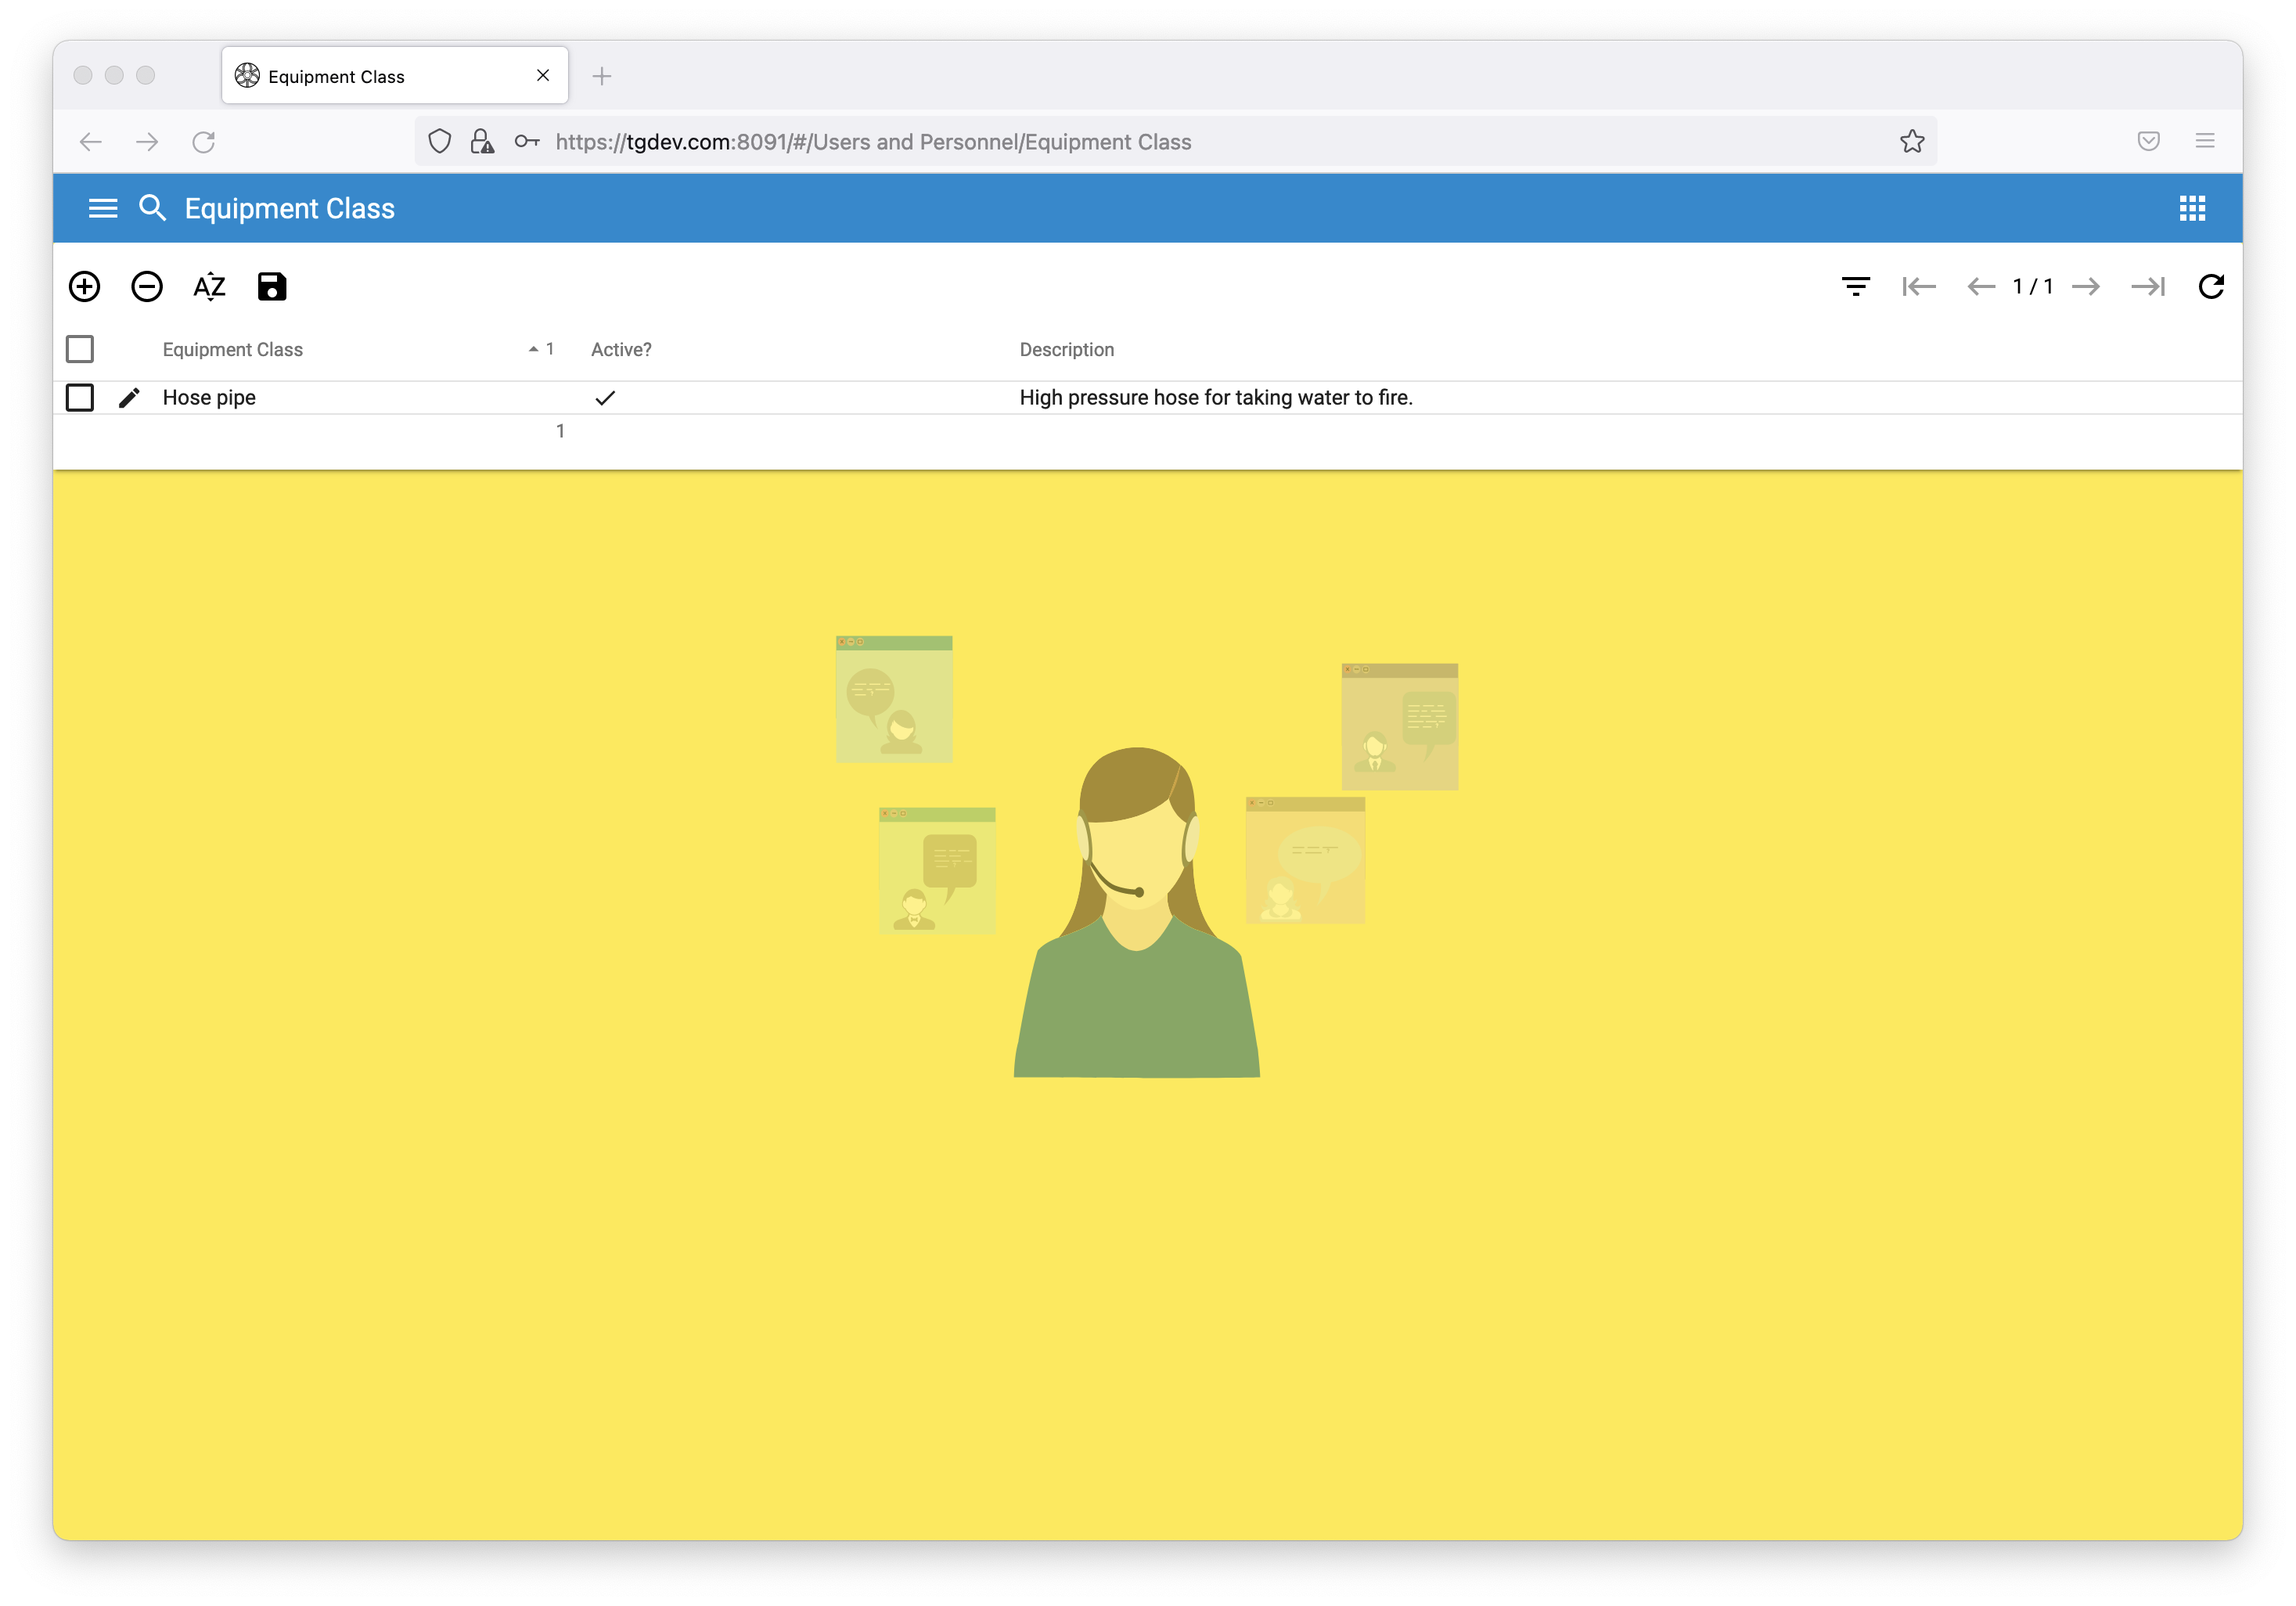
\includegraphics[width=0.95\linewidth]{sections/equipment/images/Fig.3.png}
	\caption{Equipment class search results.}\label{sections/equipment/images/Fig.3}
	\end{figure}
	
\newpage
Users can edit existing equipment classes. On the 'Main' tab, displayed on \hyperref[sections/equipment/images/Fig.4]{Fig.~\ref*{sections/equipment/images/Fig.4}}, users can edit title, activity status and description of the specific equipment class.

    \begin{figure}[!htbp]
	\centering
	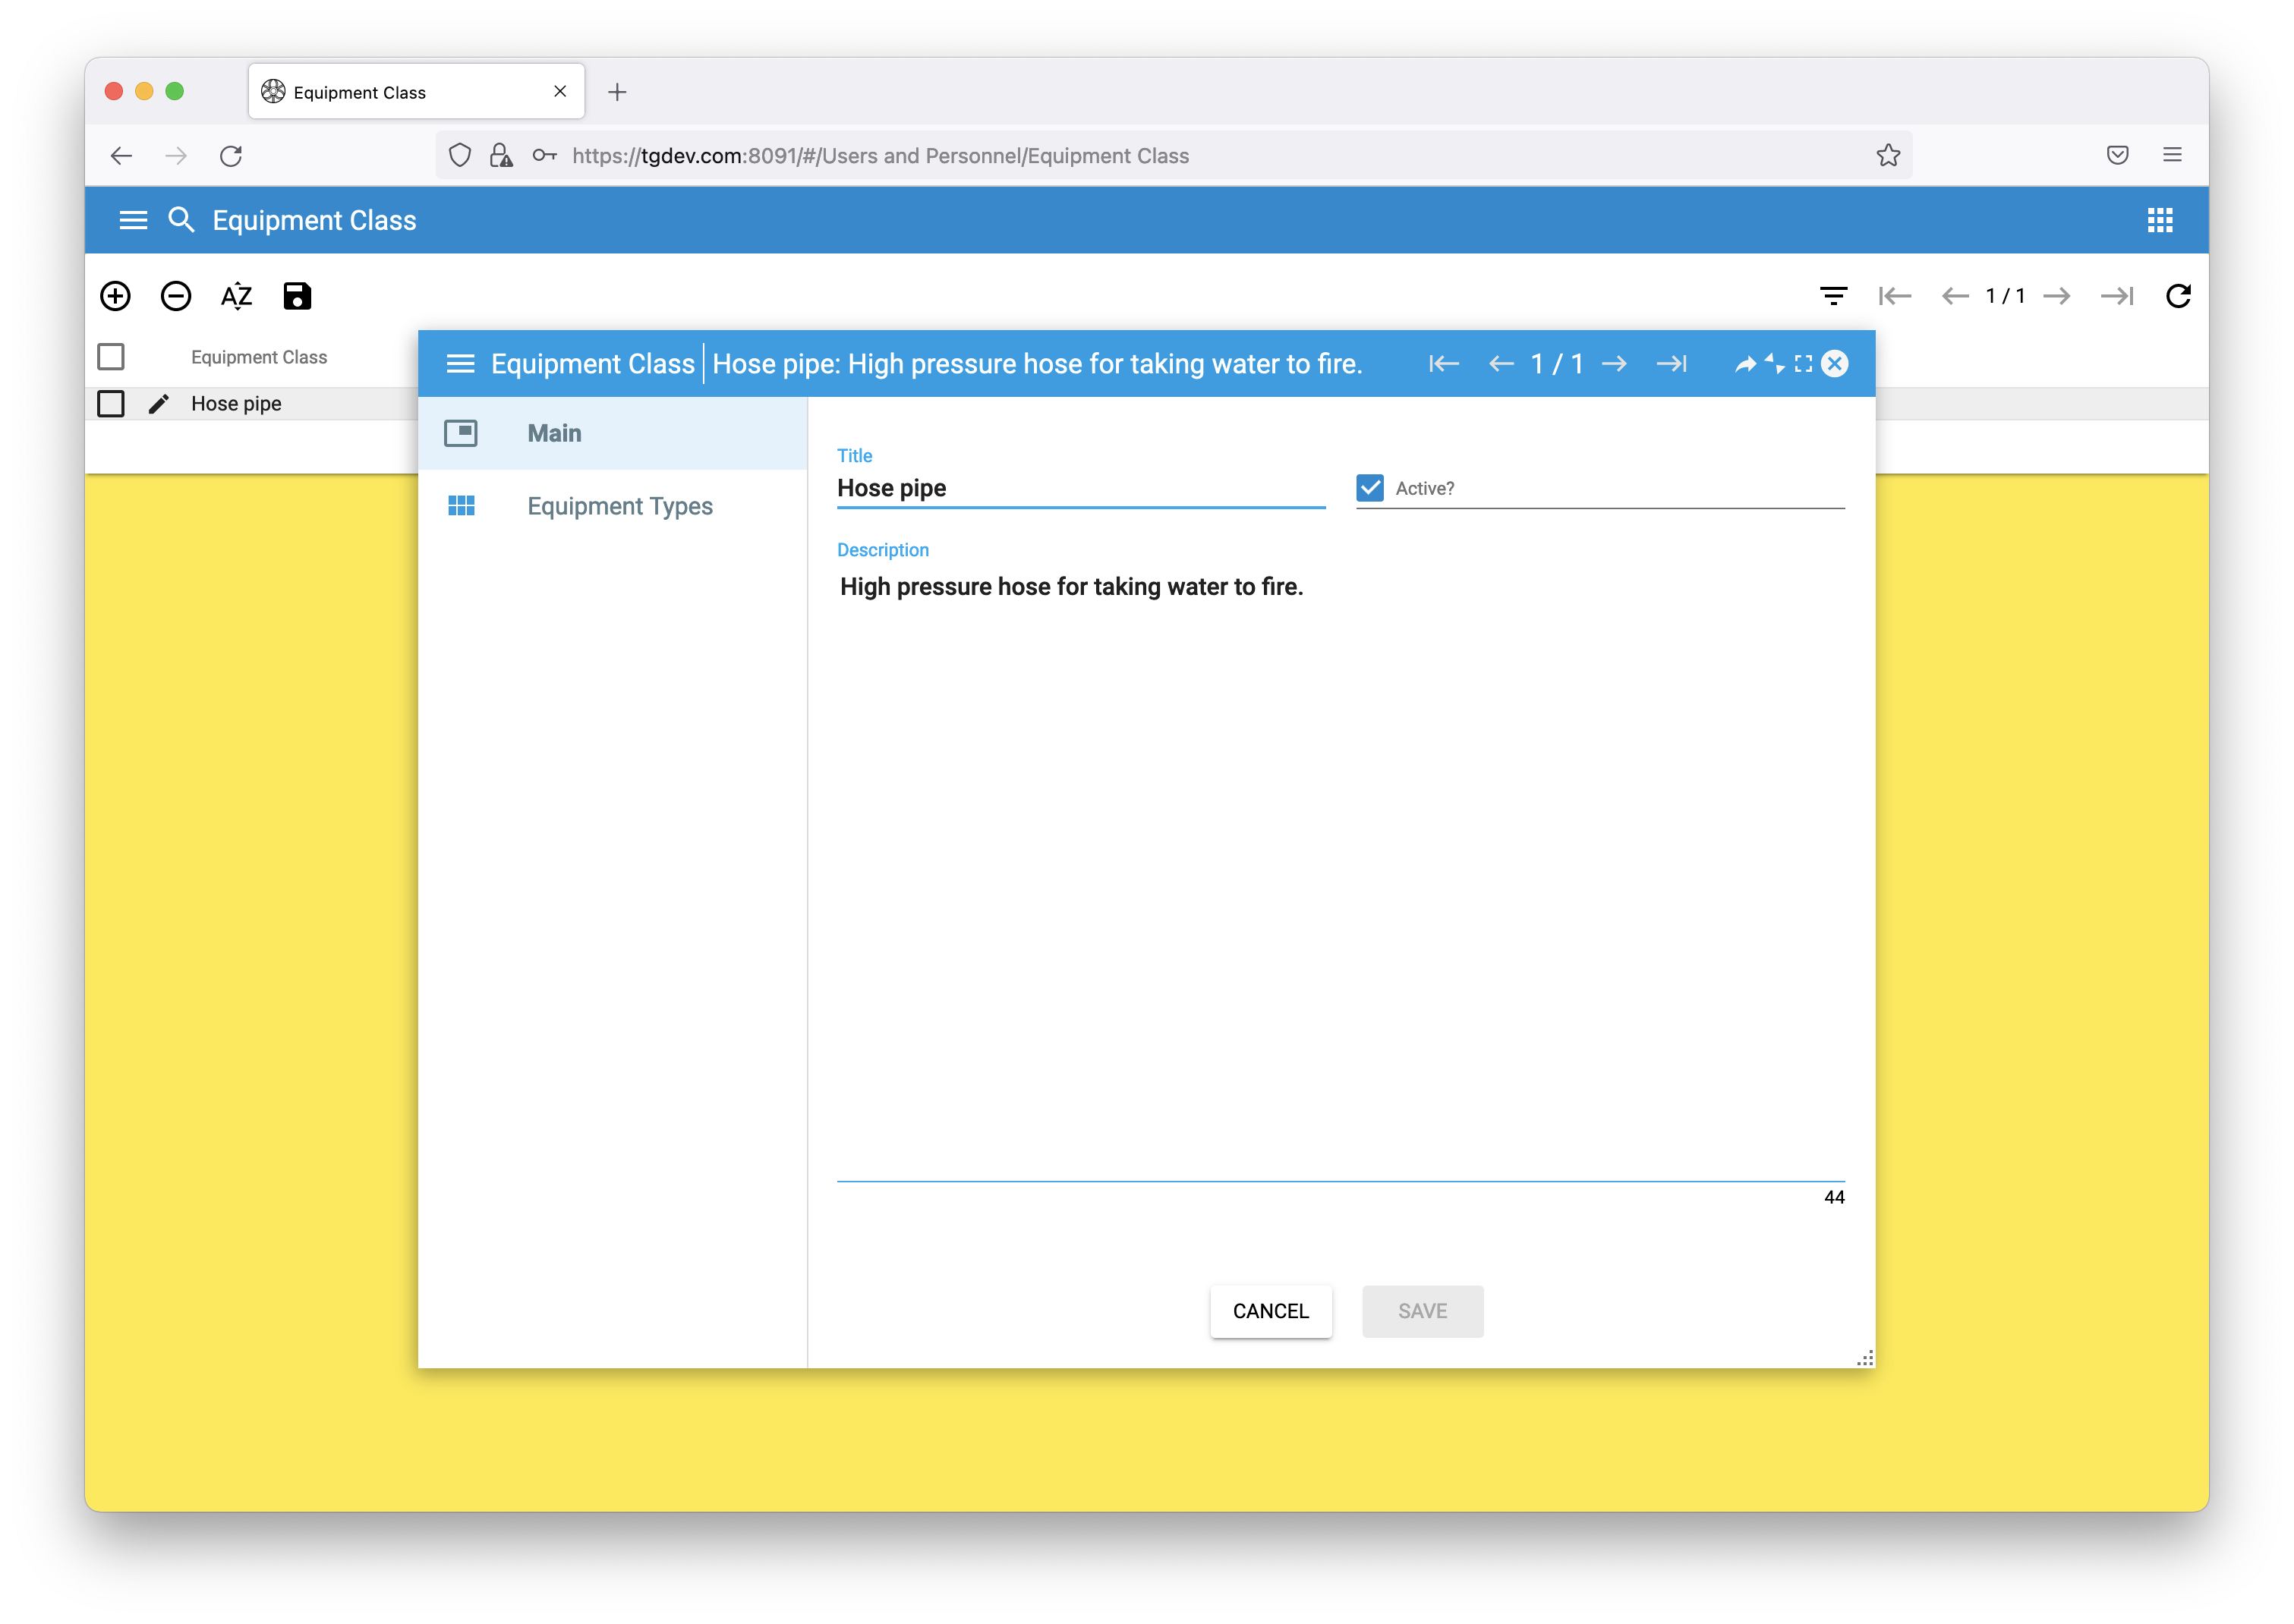
\includegraphics[width=0.95\linewidth]{sections/equipment/images/Fig.4.png}
	\caption{Equipment class editing.}\label{sections/equipment/images/Fig.4}
	\end{figure}

\newpage
On the ‘Equipment Types’ tab, users can:
\begin{itemize}
    \item observe all of the equipment types related only to this specific equipment class along with title, activity status and description, as displayed on \hyperref[sections/equipment/images/Fig.5]{Fig.~\ref*{sections/equipment/images/Fig.5}};
\end{itemize}

    \begin{figure}[!htbp]
	\centering
	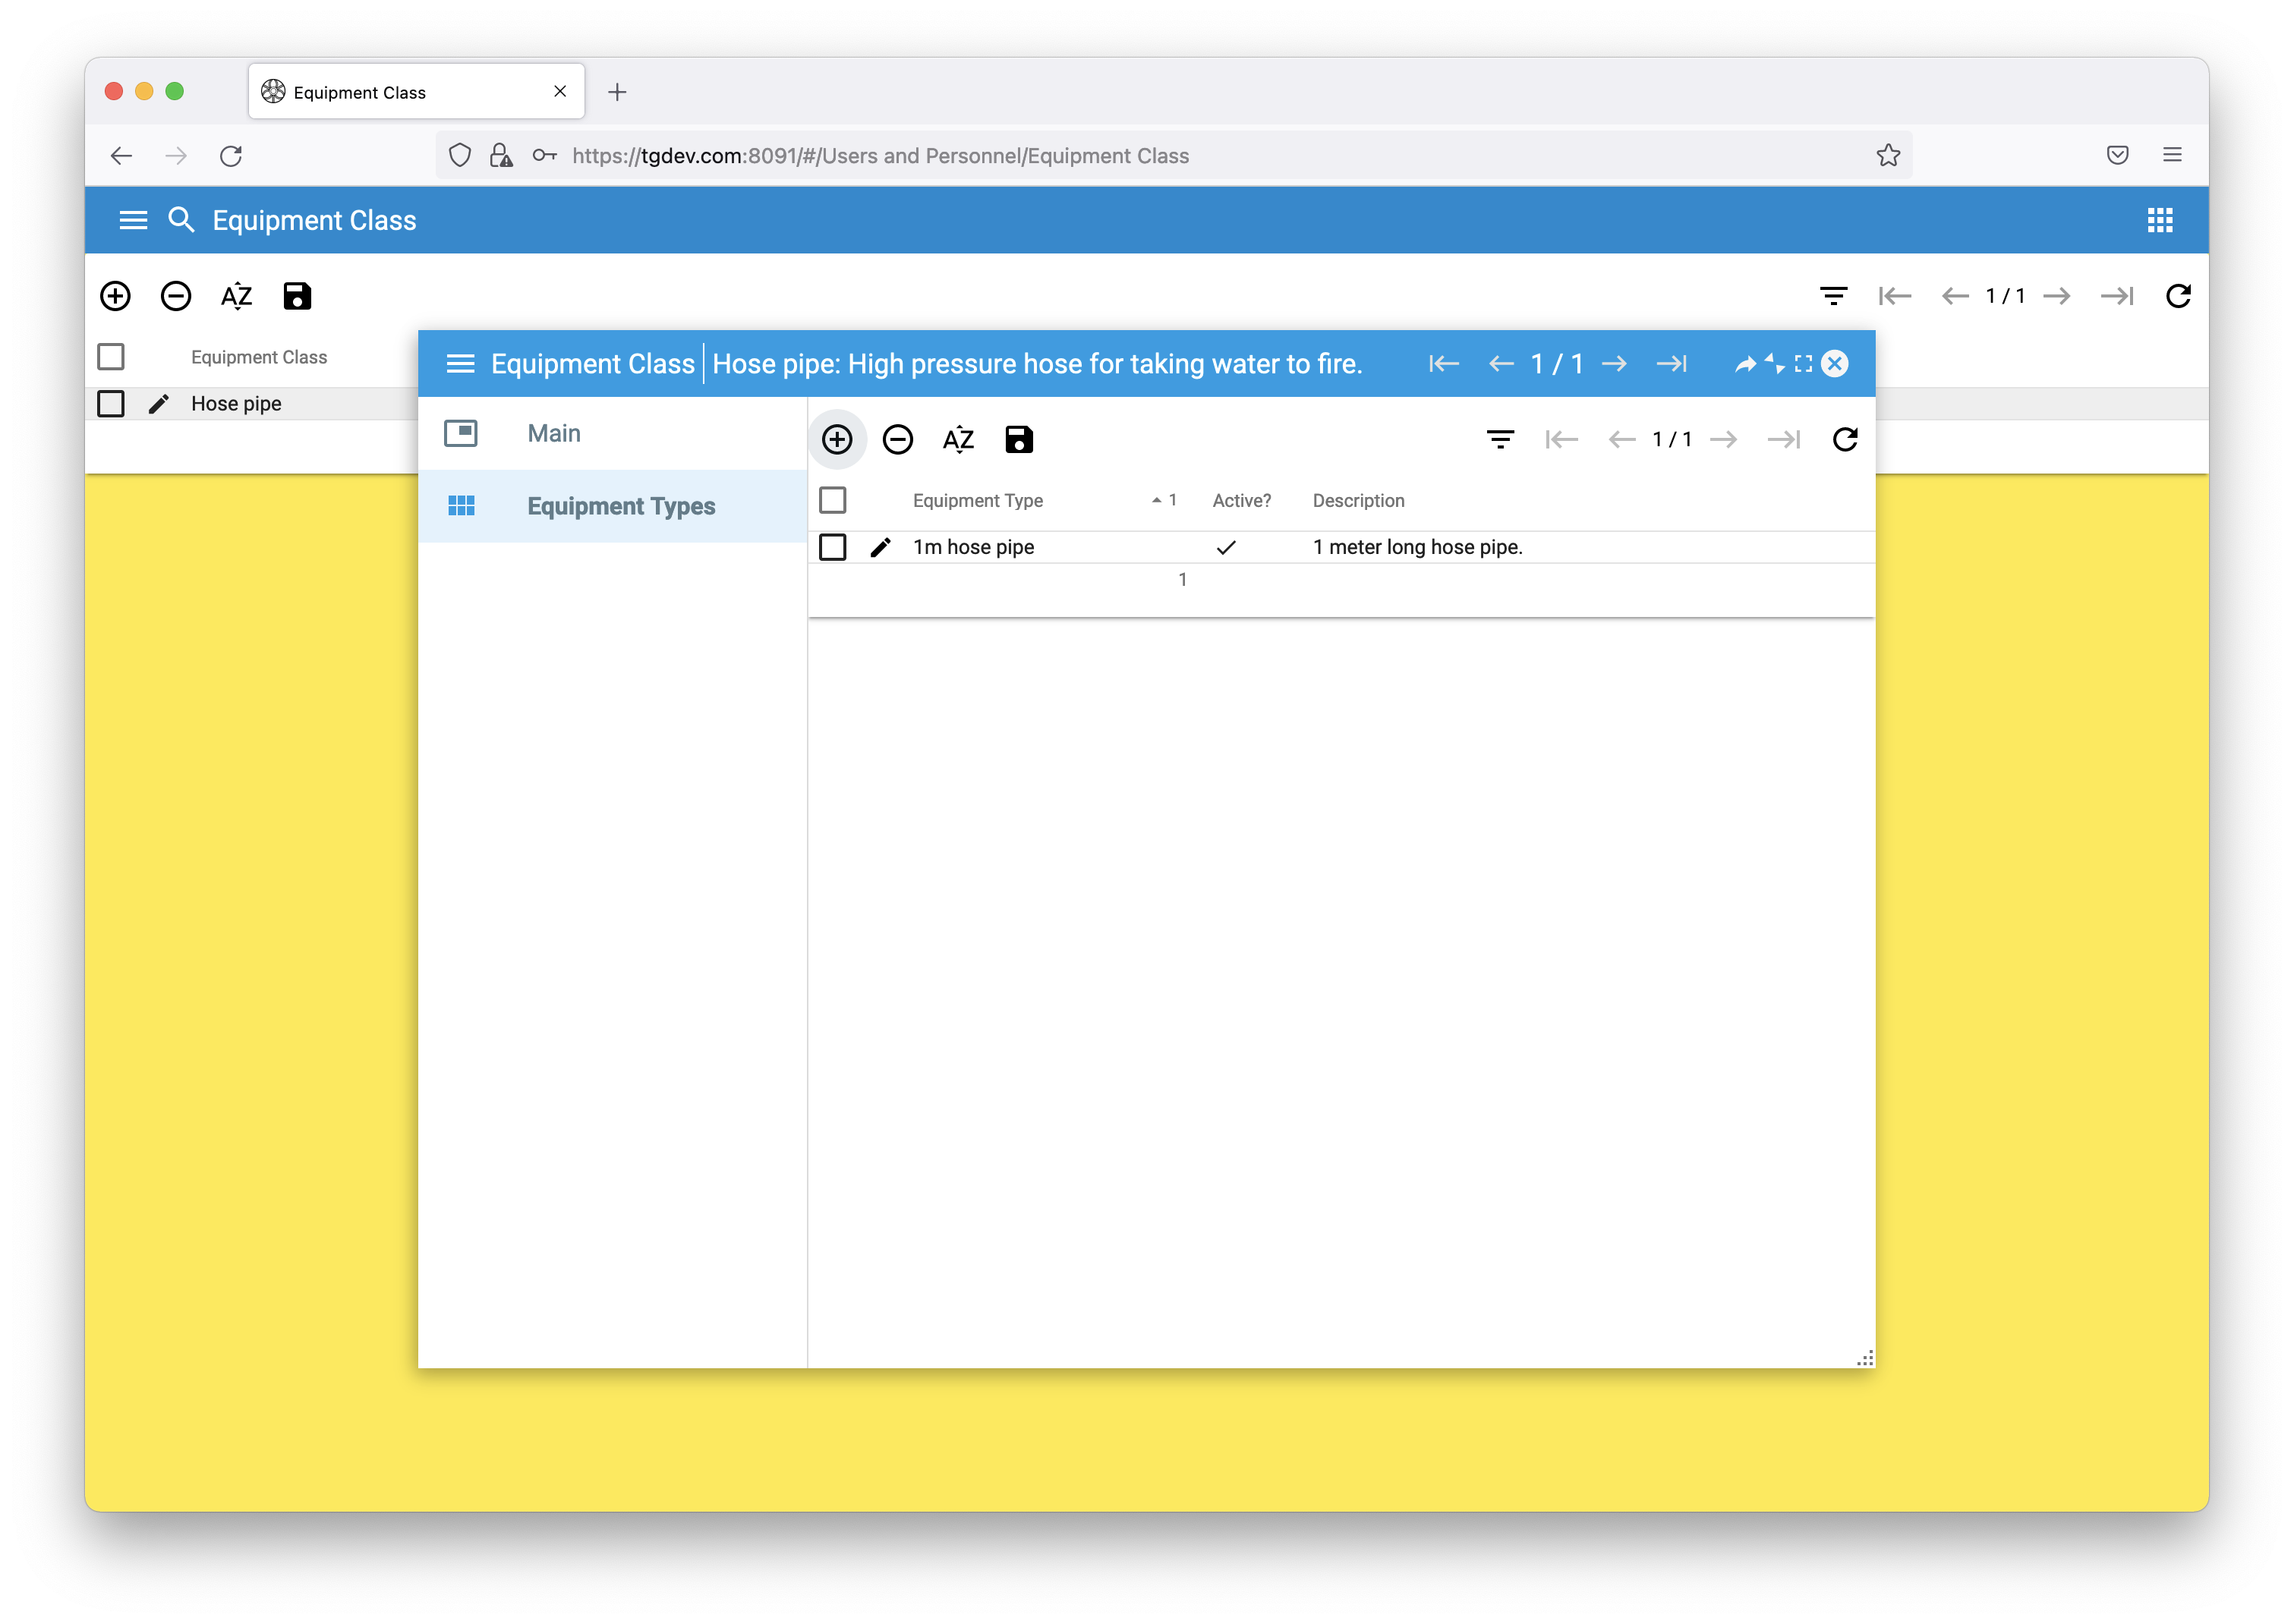
\includegraphics[width=0.95\linewidth]{sections/equipment/images/Fig.5.png}
	\caption{Embedded equipment type search results.}\label{sections/equipment/images/Fig.5}
	\end{figure}
	
\newpage
\begin{itemize}
    \item search for existing equipment types related only to this specific equipment class either by specifying title, which is auto-completed, or activity status, or both, as displayed on \hyperref[sections/equipment/images/Fig.6]{Fig.~\ref*{sections/equipment/images/Fig.6}};
\end{itemize}

    \begin{figure}[!htbp]
	\centering
	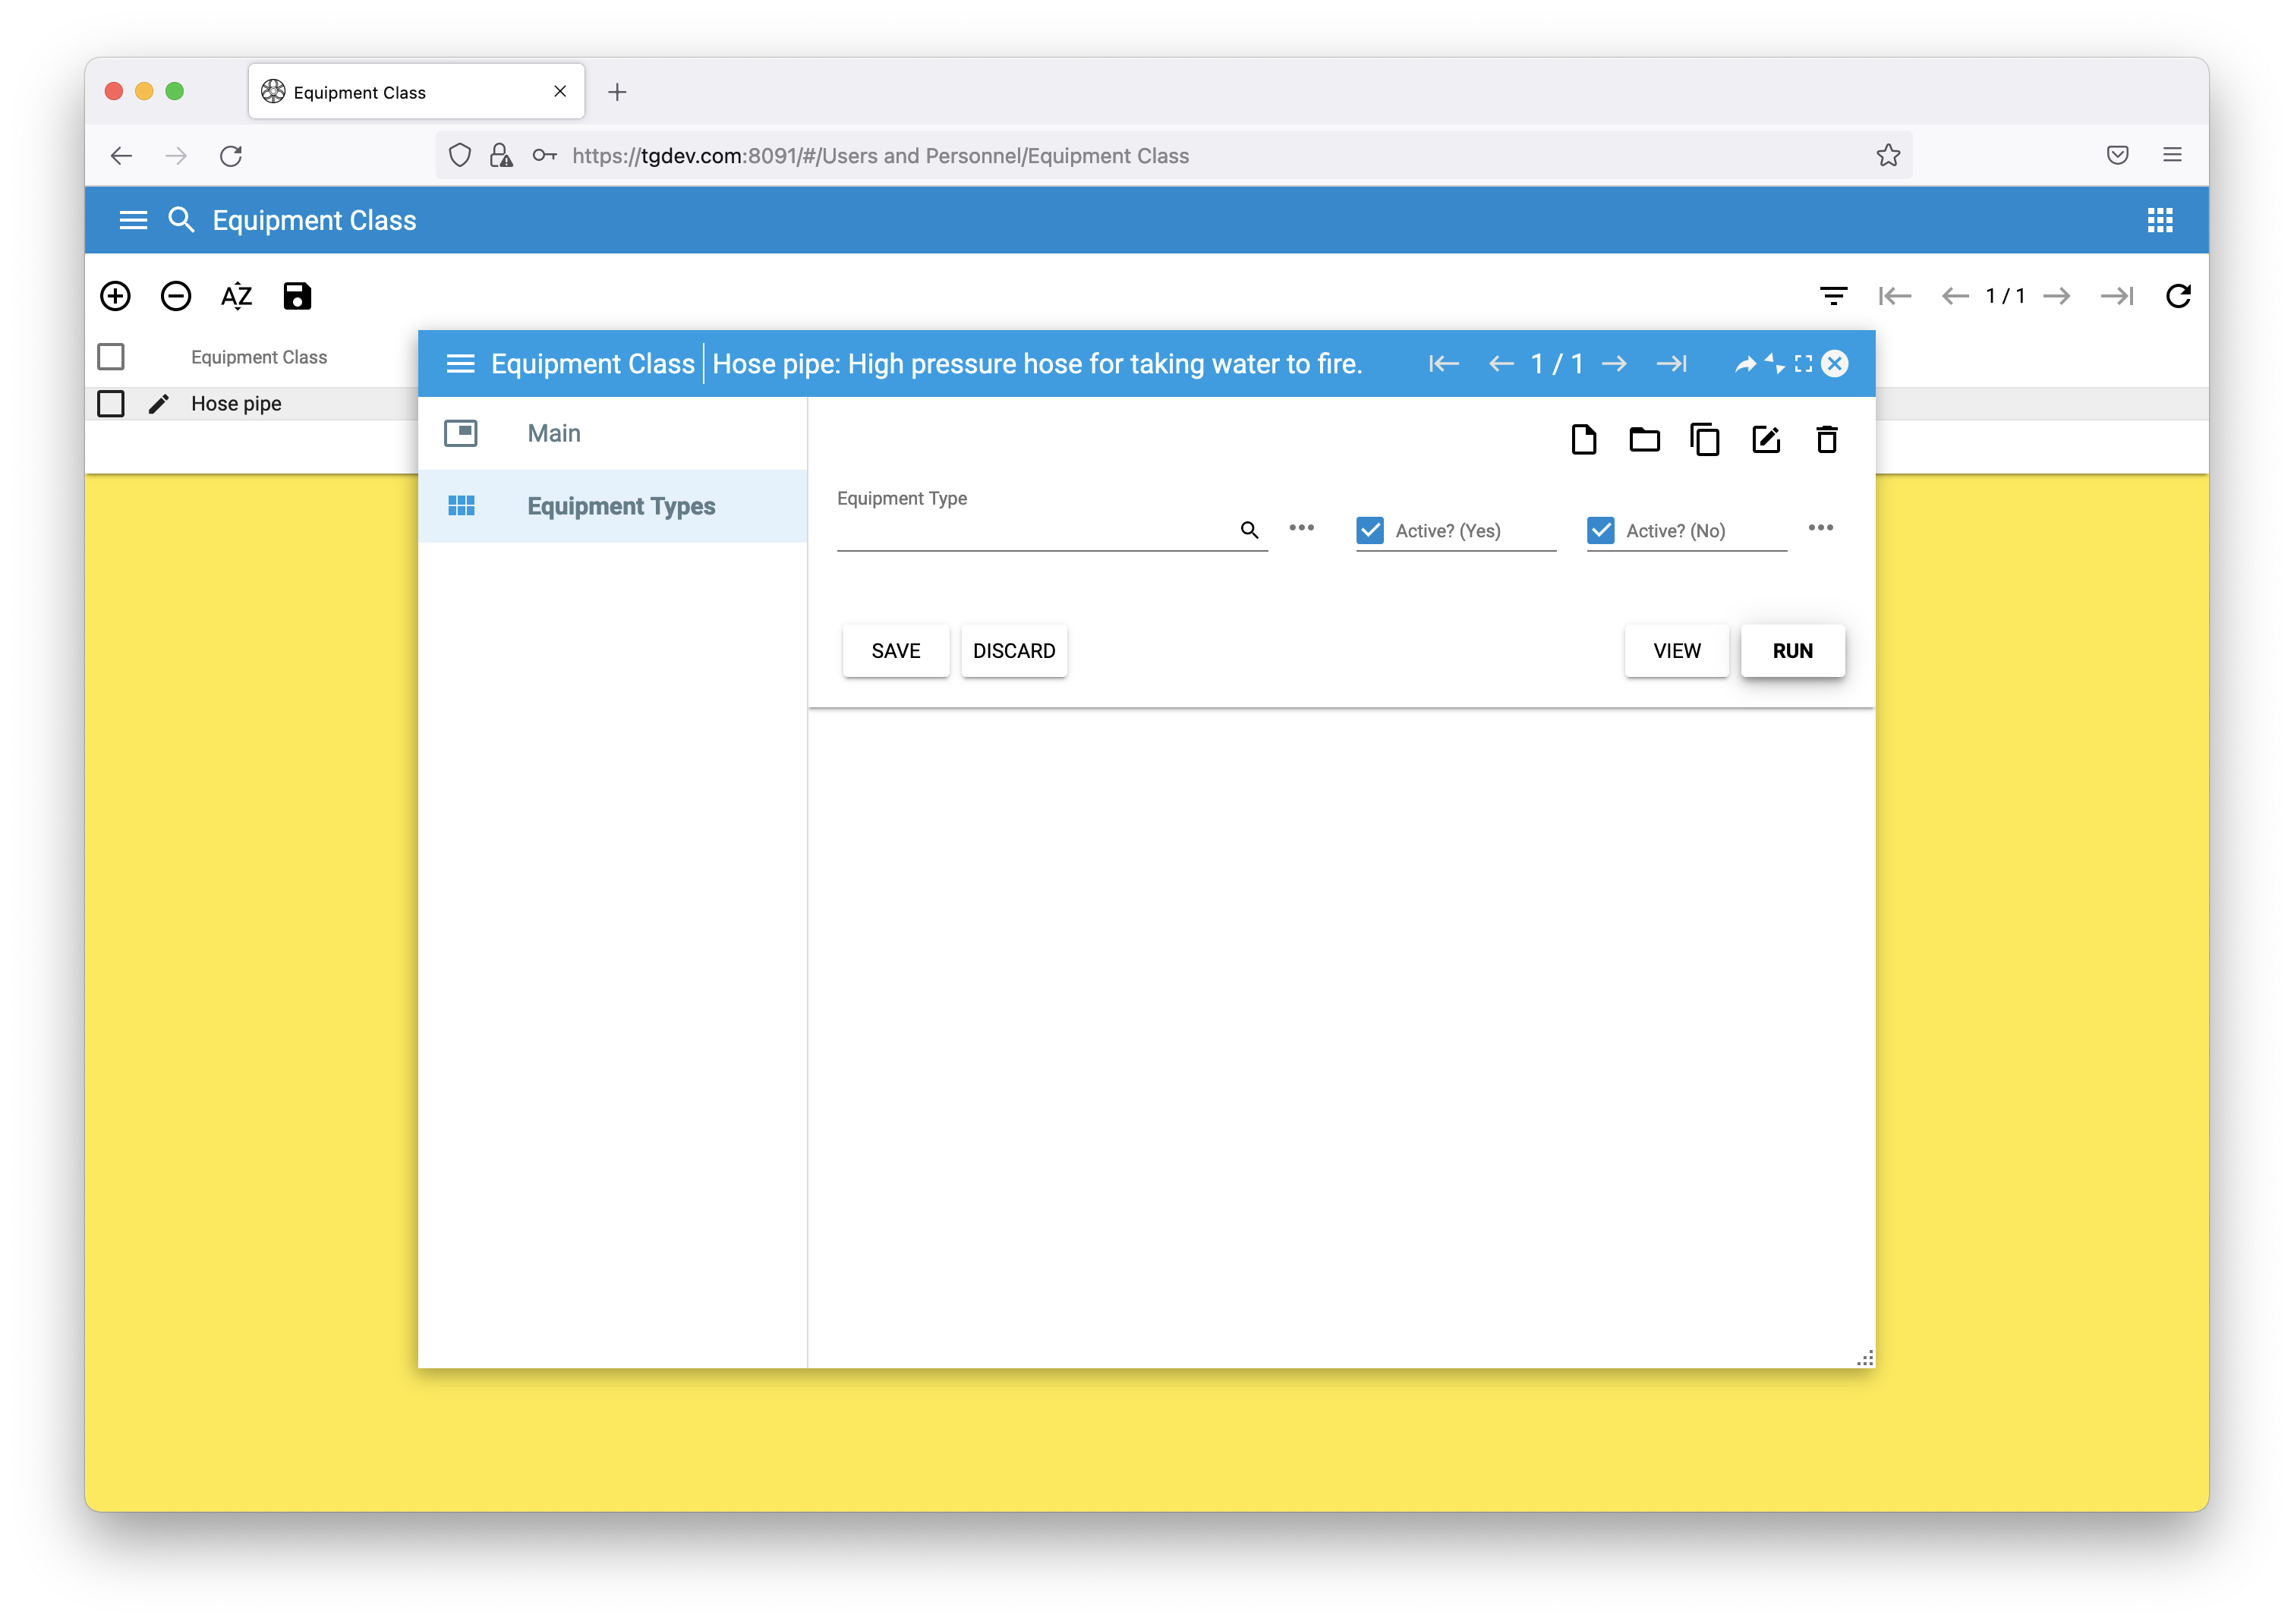
\includegraphics[width=0.95\linewidth]{sections/equipment/images/Fig.6.png}
	\caption{Embedded equipment type search query.}\label{sections/equipment/images/Fig.6}
	\end{figure}
	
\newpage
\begin{itemize}
    \item create equipment type by filling in its title without white spaces and activity status, as well as its description, as displayed on \hyperref[sections/equipment/images/Fig.7]{Fig.~\ref*{sections/equipment/images/Fig.7}}. Equipment class field is automatically auto-completed with this specific equipment class.
\end{itemize}

    \begin{figure}[!htbp]
	\centering
	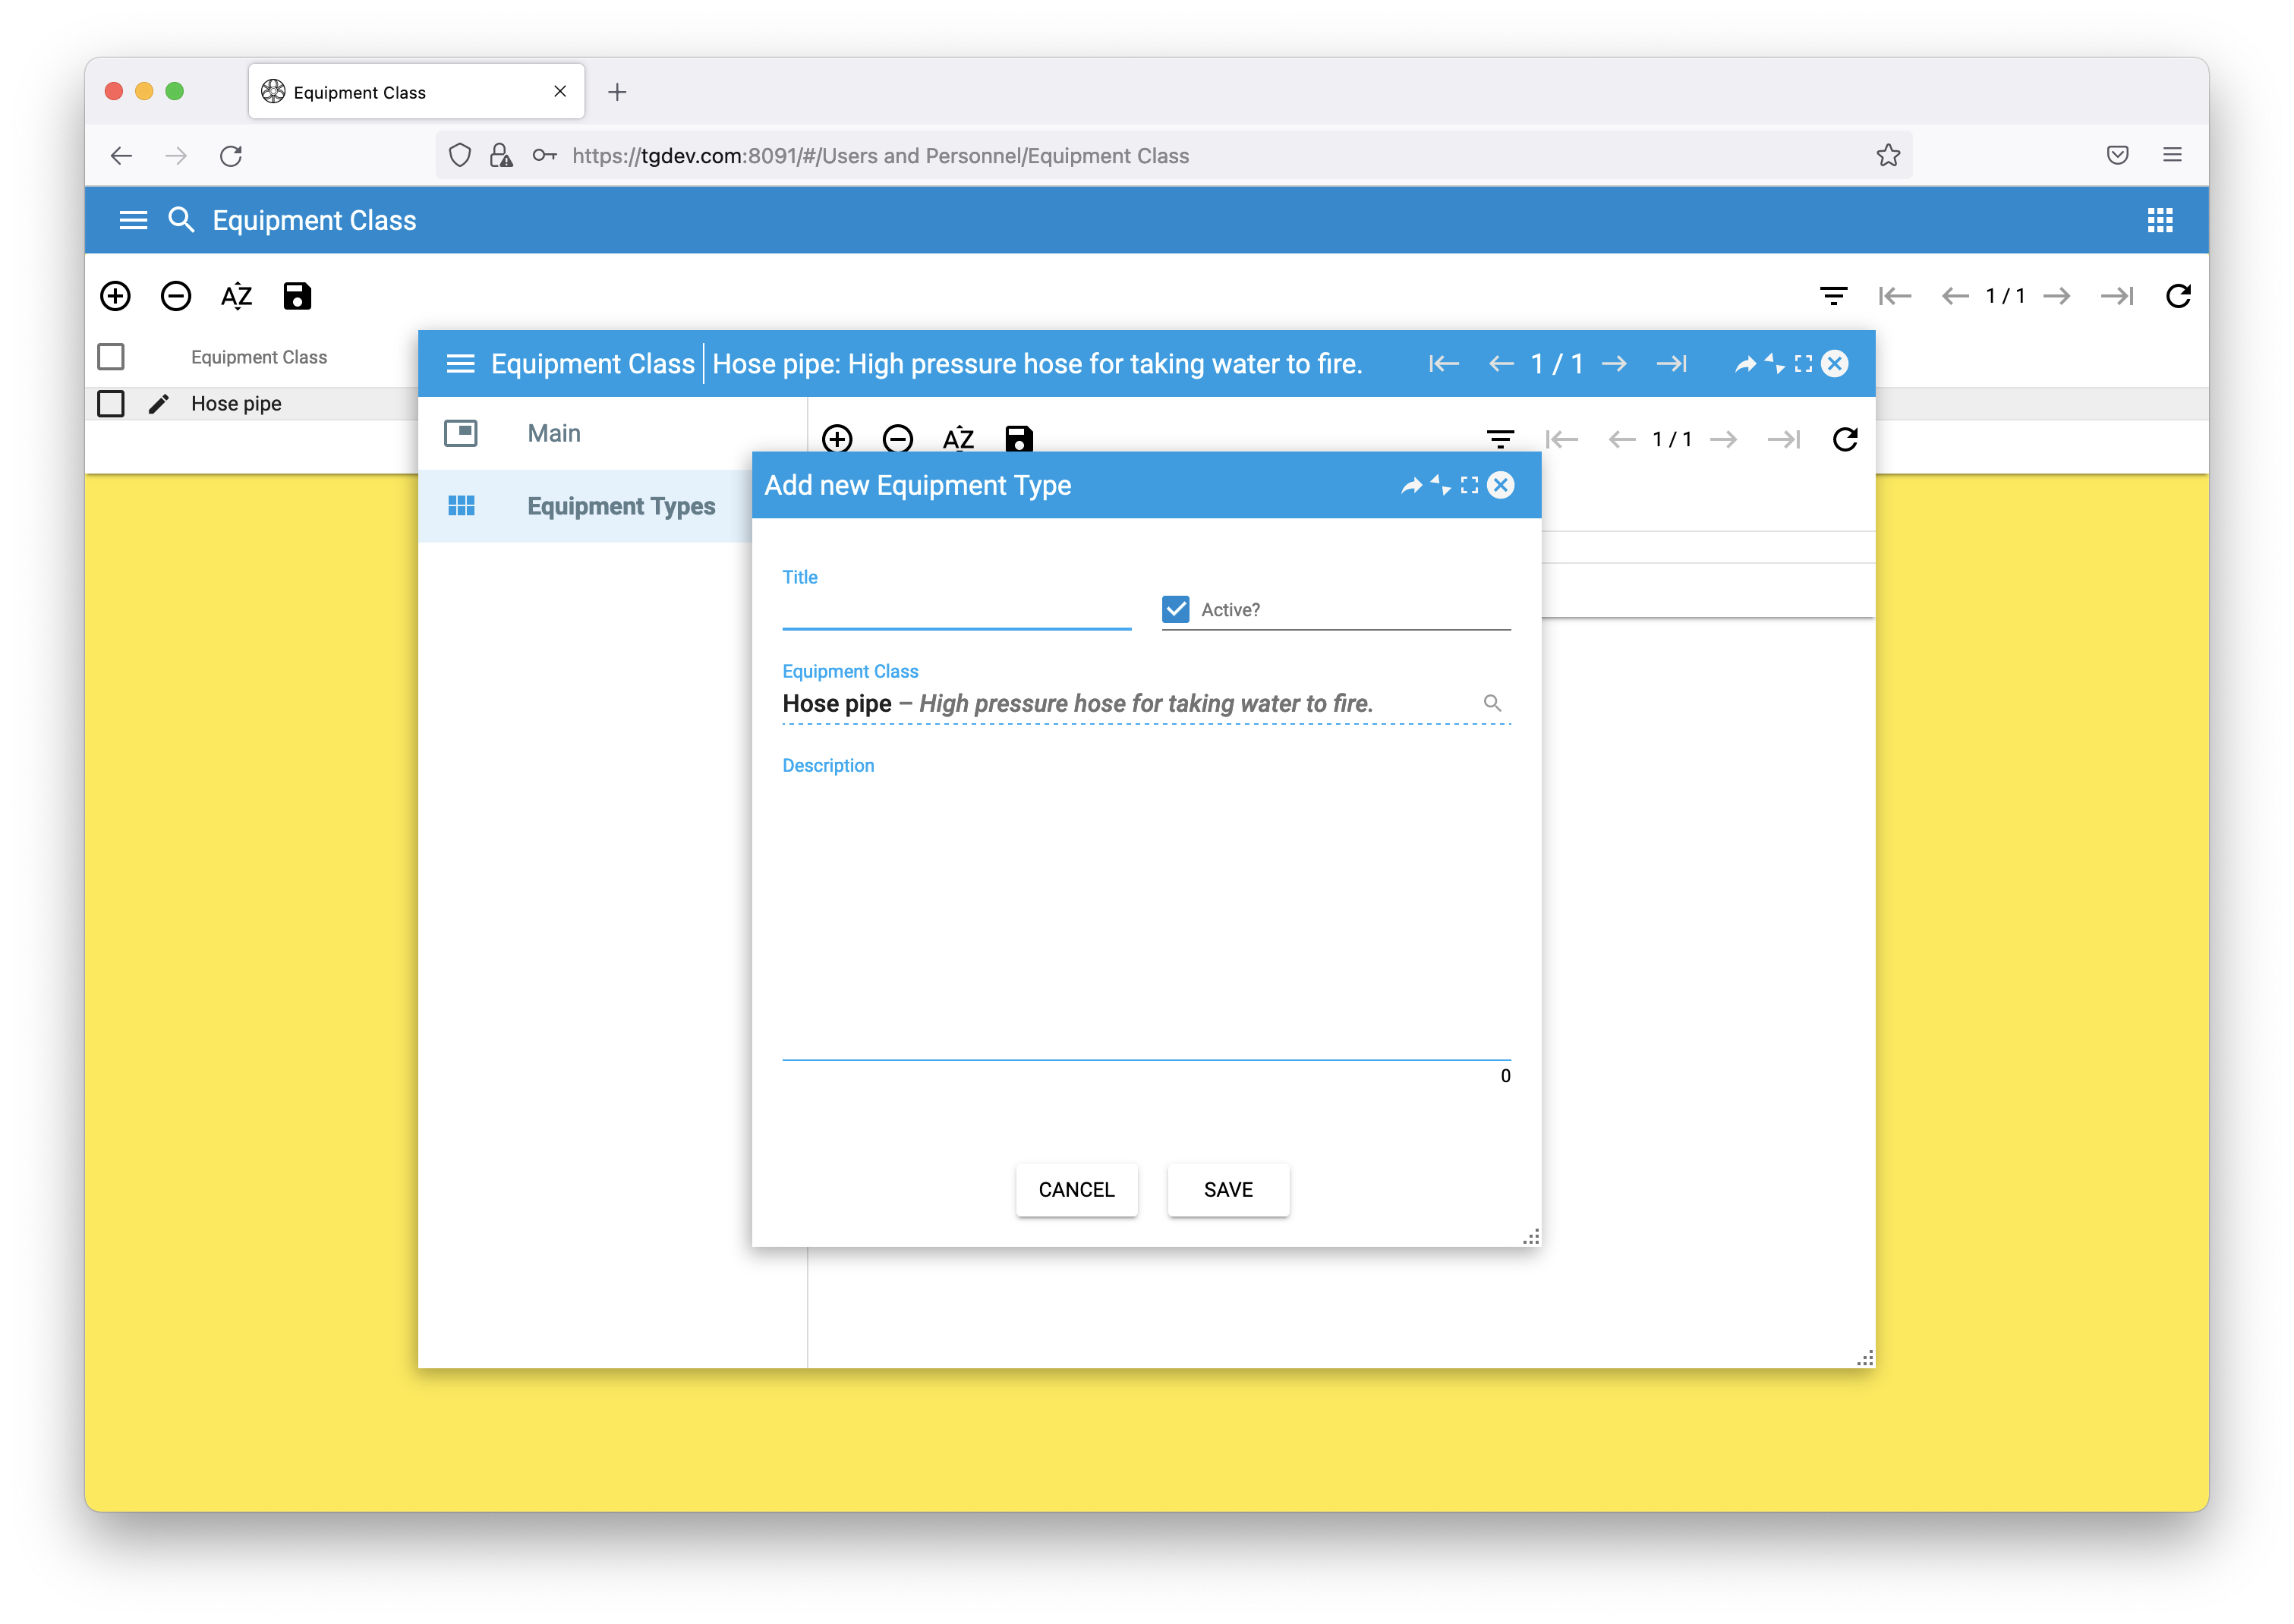
\includegraphics[width=0.95\linewidth]{sections/equipment/images/Fig.7.png}
	\caption{Embedded equipment type creation.}\label{sections/equipment/images/Fig.7}
	\end{figure}

\newpage	
\subsection{Equipment Type}

In order to perform classification of equipment in more detail correctly, users can create equipment types. Possible equipment types are 1m hose pipe, assault ladder, electric lamp, etc. When creating a new equipment type, users have to fill in its title without white spaces, activity status, equipment class it belongs to, which is auto-completed, as well as its description, as displayed on \hyperref[sections/equipment/images/Fig.8]{Fig.~\ref*{sections/equipment/images/Fig.8}}. 

    \begin{figure}[!htbp]
	\centering
	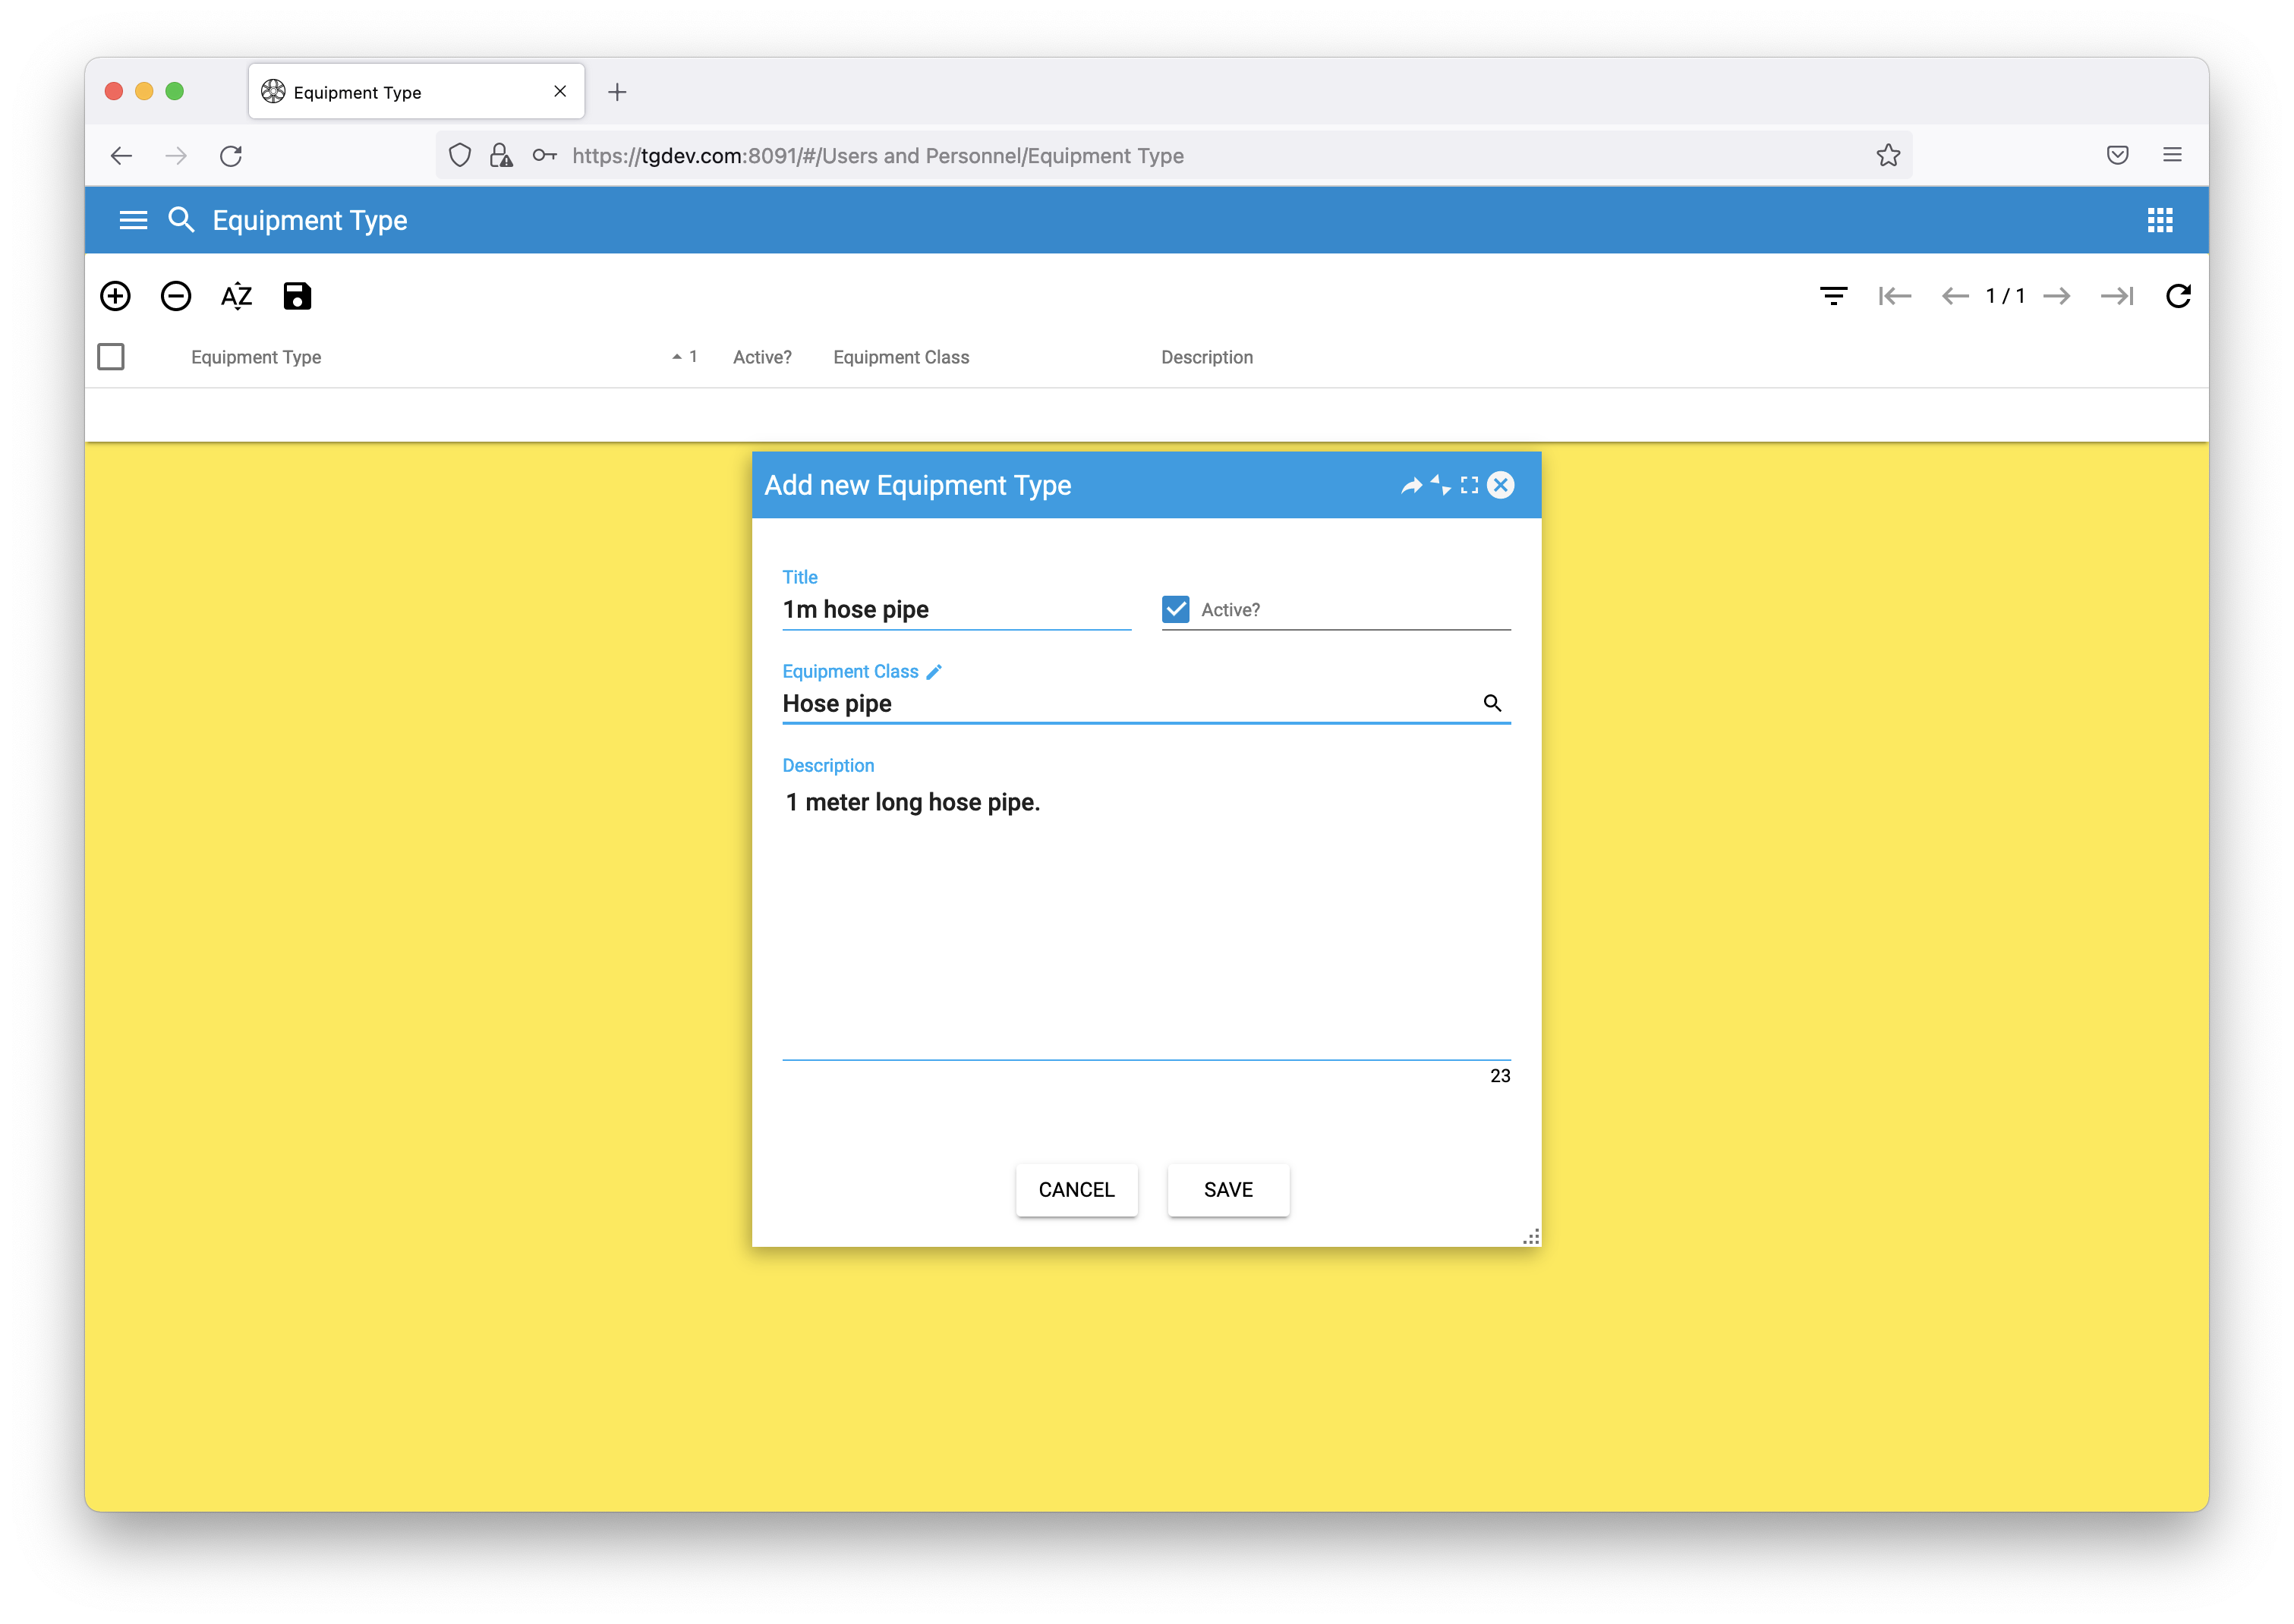
\includegraphics[width=0.95\linewidth]{sections/equipment/images/Fig.8.png}
	\caption{Equipment type creation.}\label{sections/equipment/images/Fig.8}
	\end{figure}

\newpage
Users can search for existing equipment types either by specifying title, which is auto-completed, activity status, equipment class they belong to, or all, as displayed on \hyperref[sections/equipment/images/Fig.9]{Fig.~\ref*{sections/equipment/images/Fig.9}}.

    \begin{figure}[!htbp]
	\centering
	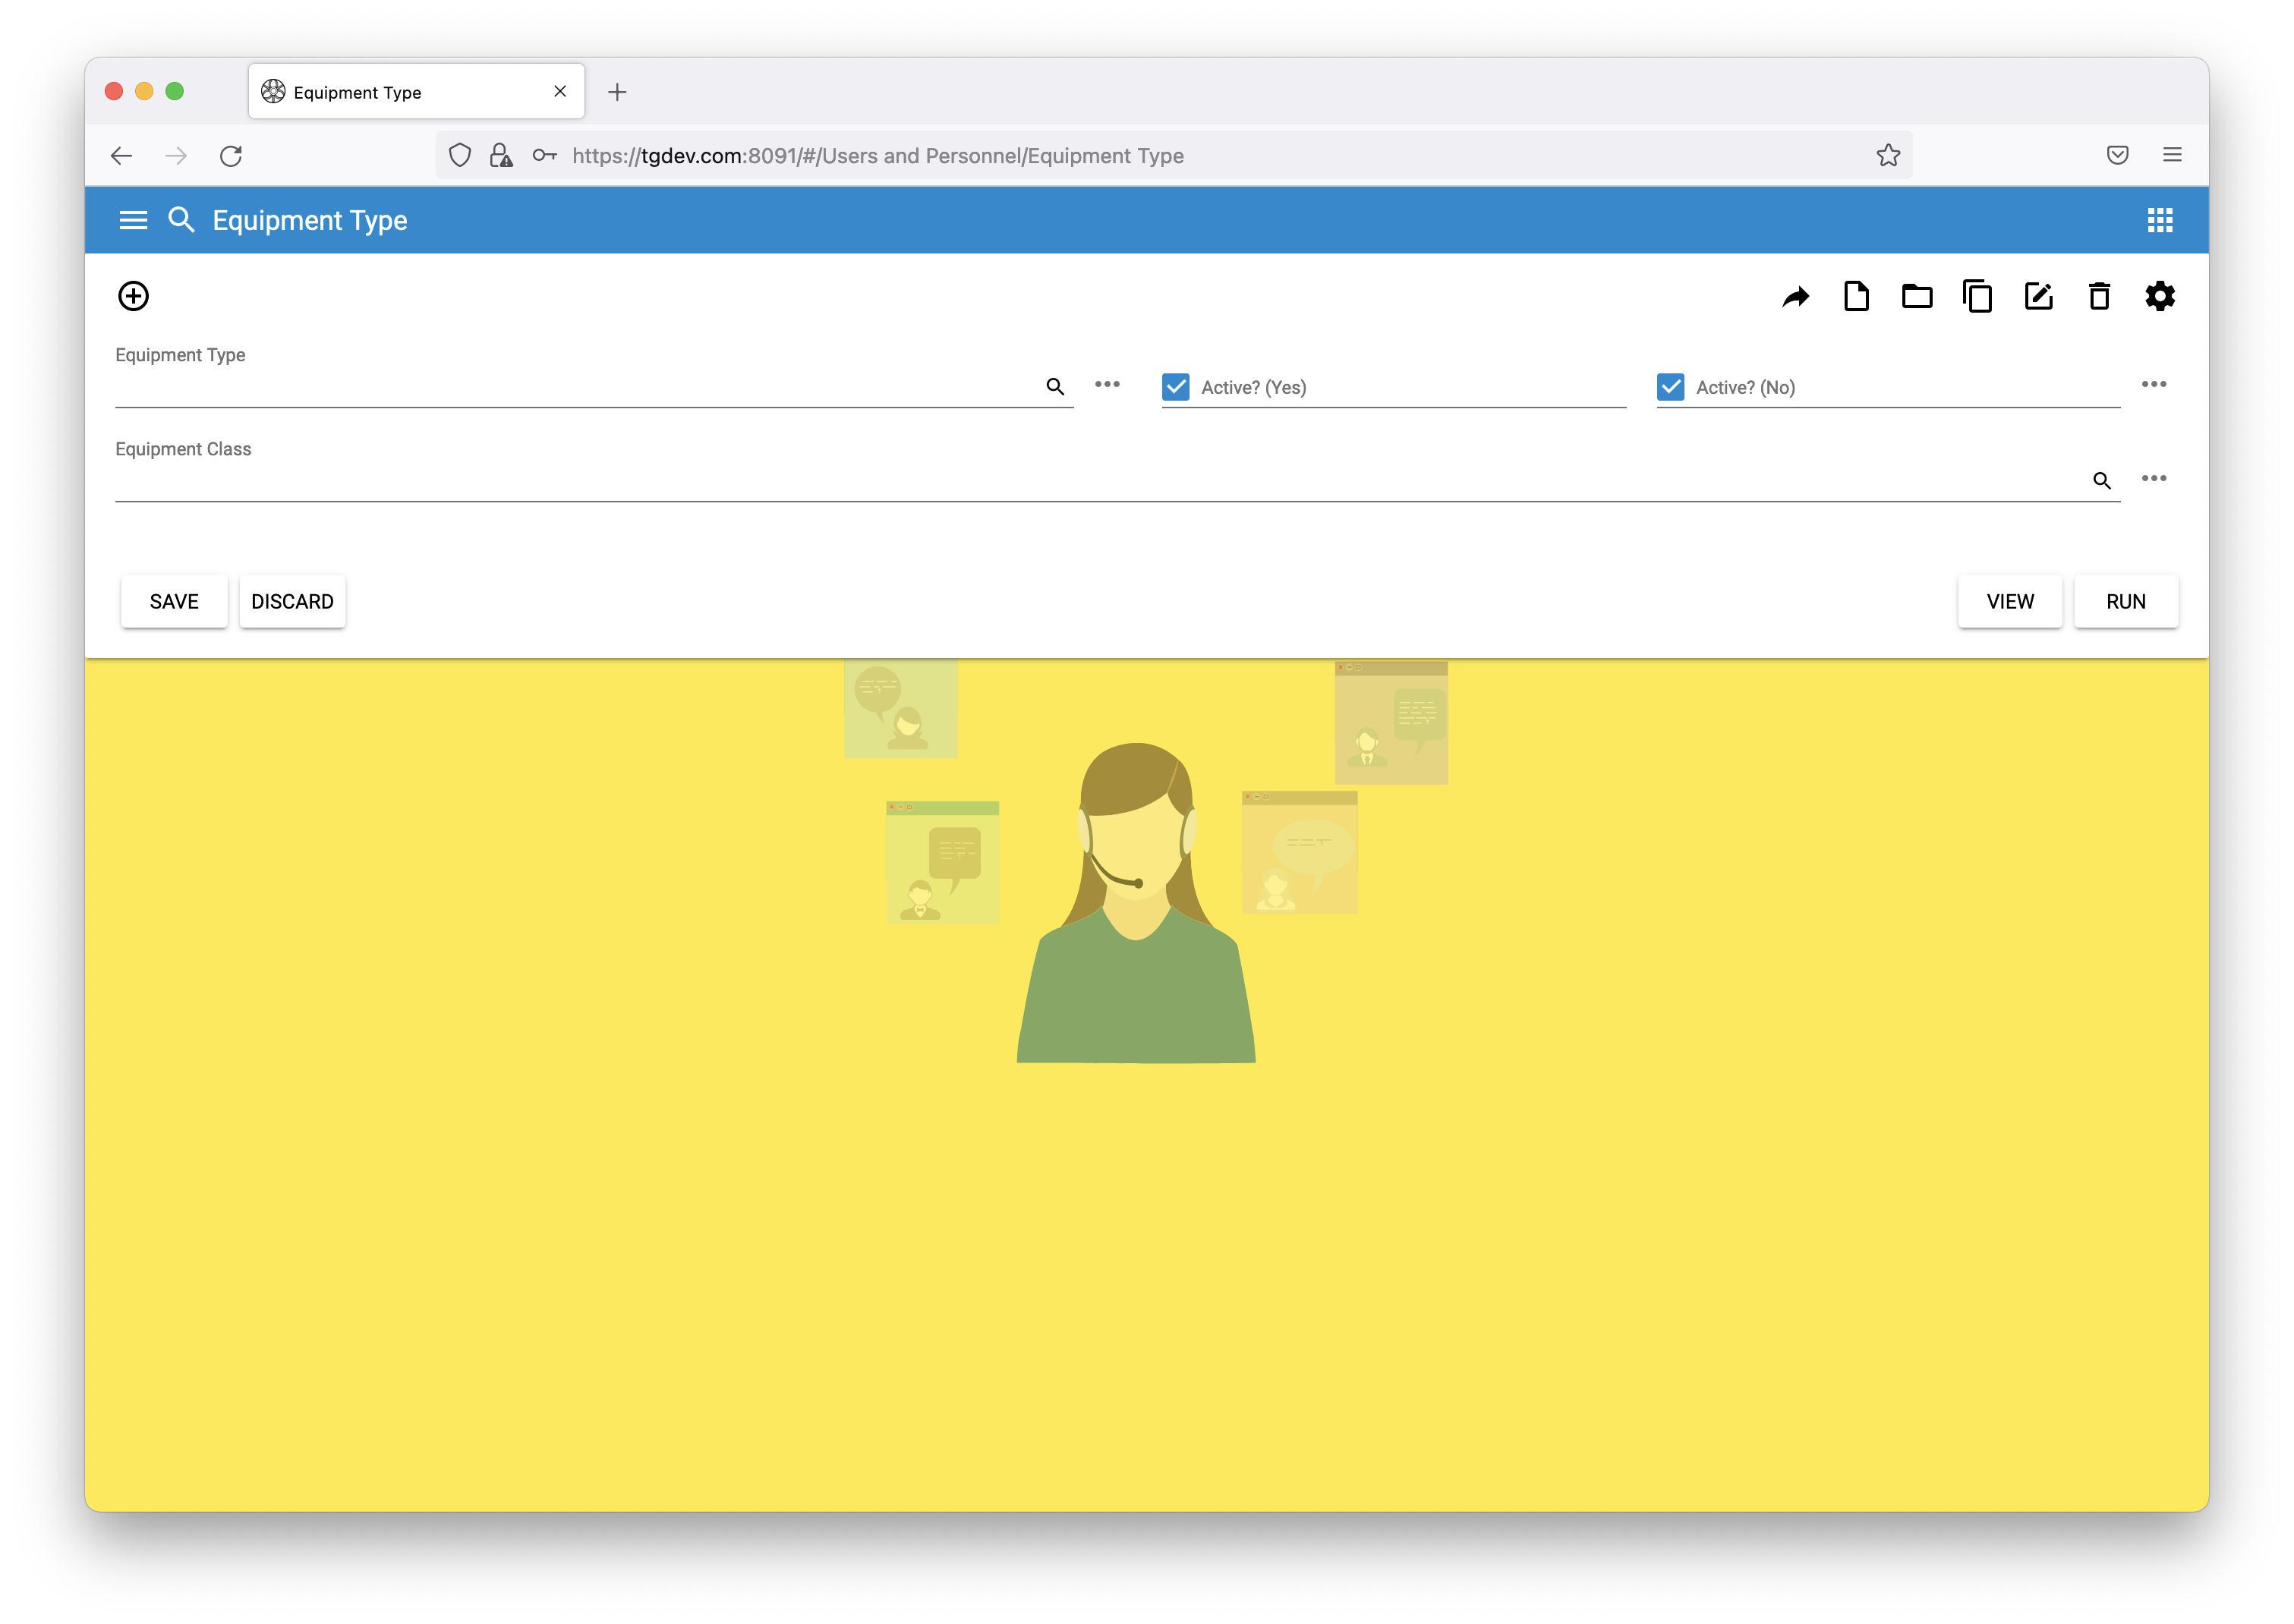
\includegraphics[width=0.95\linewidth]{sections/equipment/images/Fig.9.png}
	\caption{Equipment type search query.}\label{sections/equipment/images/Fig.9}
	\end{figure}
	
\newpage
Search results are displayed along with title, activity status, equipment class and description of the equipment type, as displayed on \hyperref[sections/equipment/images/Fig.10]{Fig.~\ref*{sections/equipment/images/Fig.10}}.

    \begin{figure}[!htbp]
	\centering
	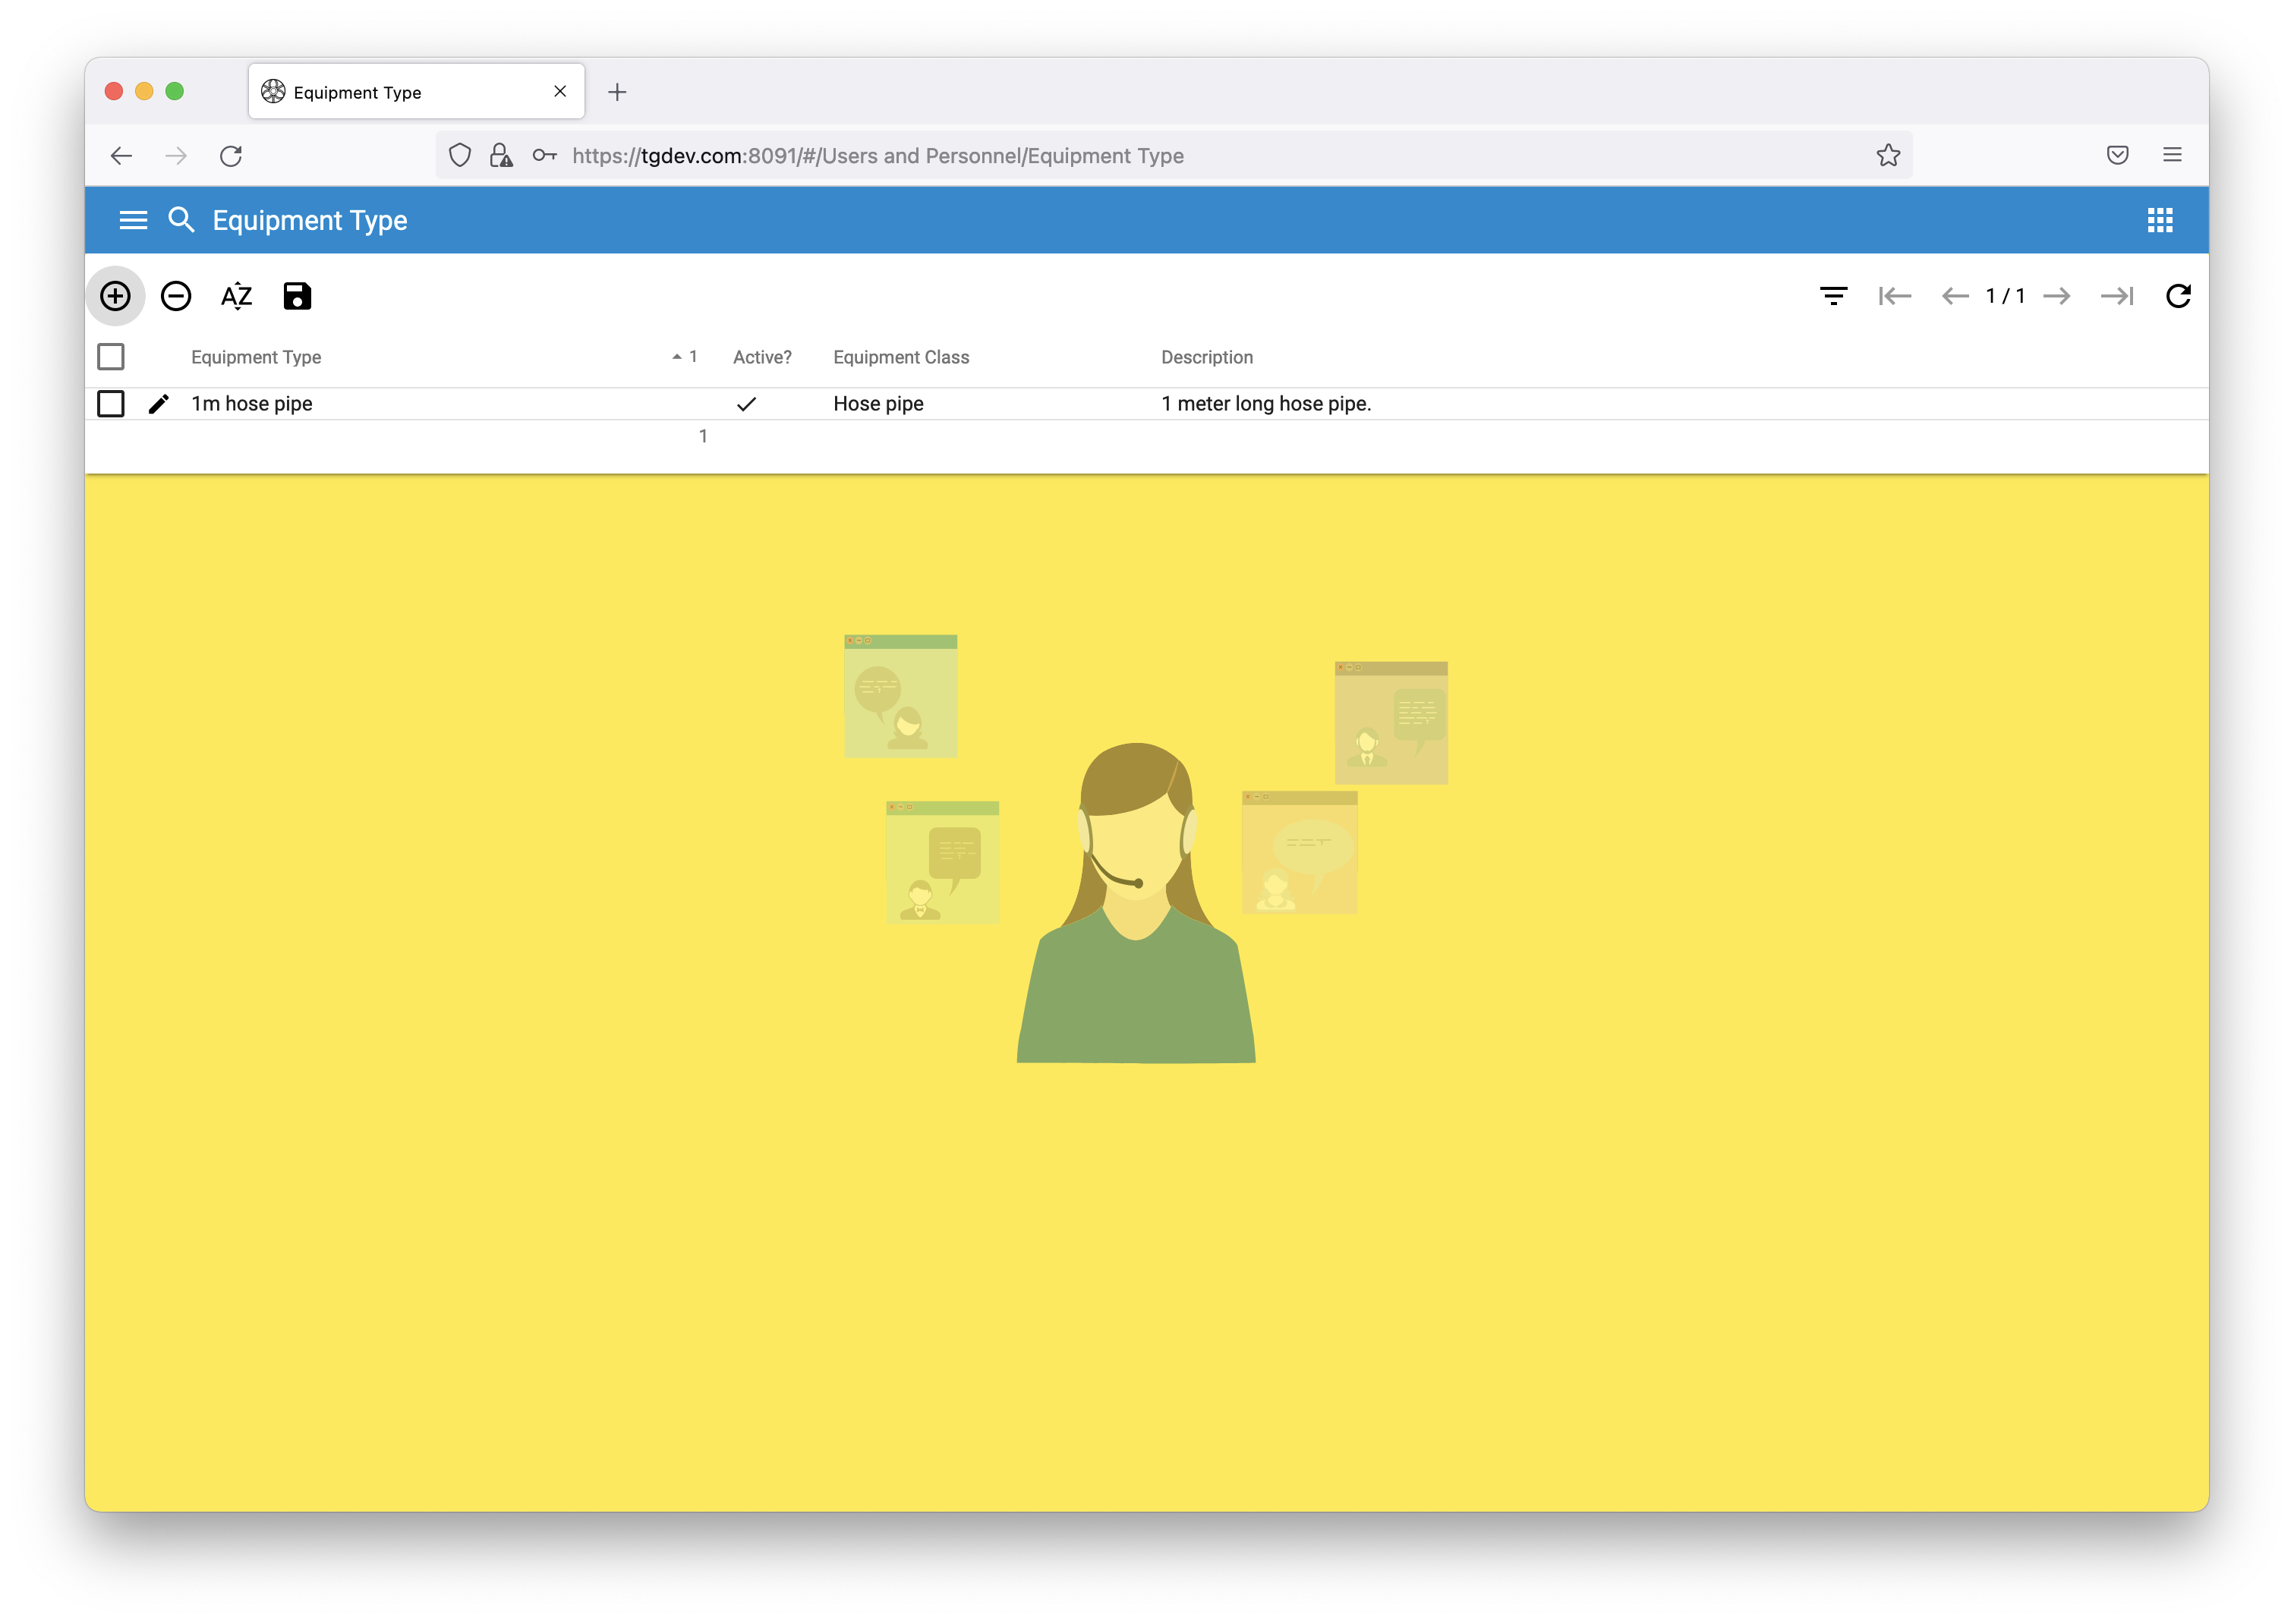
\includegraphics[width=0.95\linewidth]{sections/equipment/images/Fig.10.png}
	\caption{Equipment type search results.}\label{sections/equipment/images/Fig.10}
	\end{figure}

\newpage
Users can edit existing equipment types. As displayed on \hyperref[sections/equipment/images/Fig.11]{Fig.~\ref*{sections/equipment/images/Fig.11}}, users can edit title, activity status, equipment class and description of the specific equipment type.

    \begin{figure}[!htbp]
	\centering
	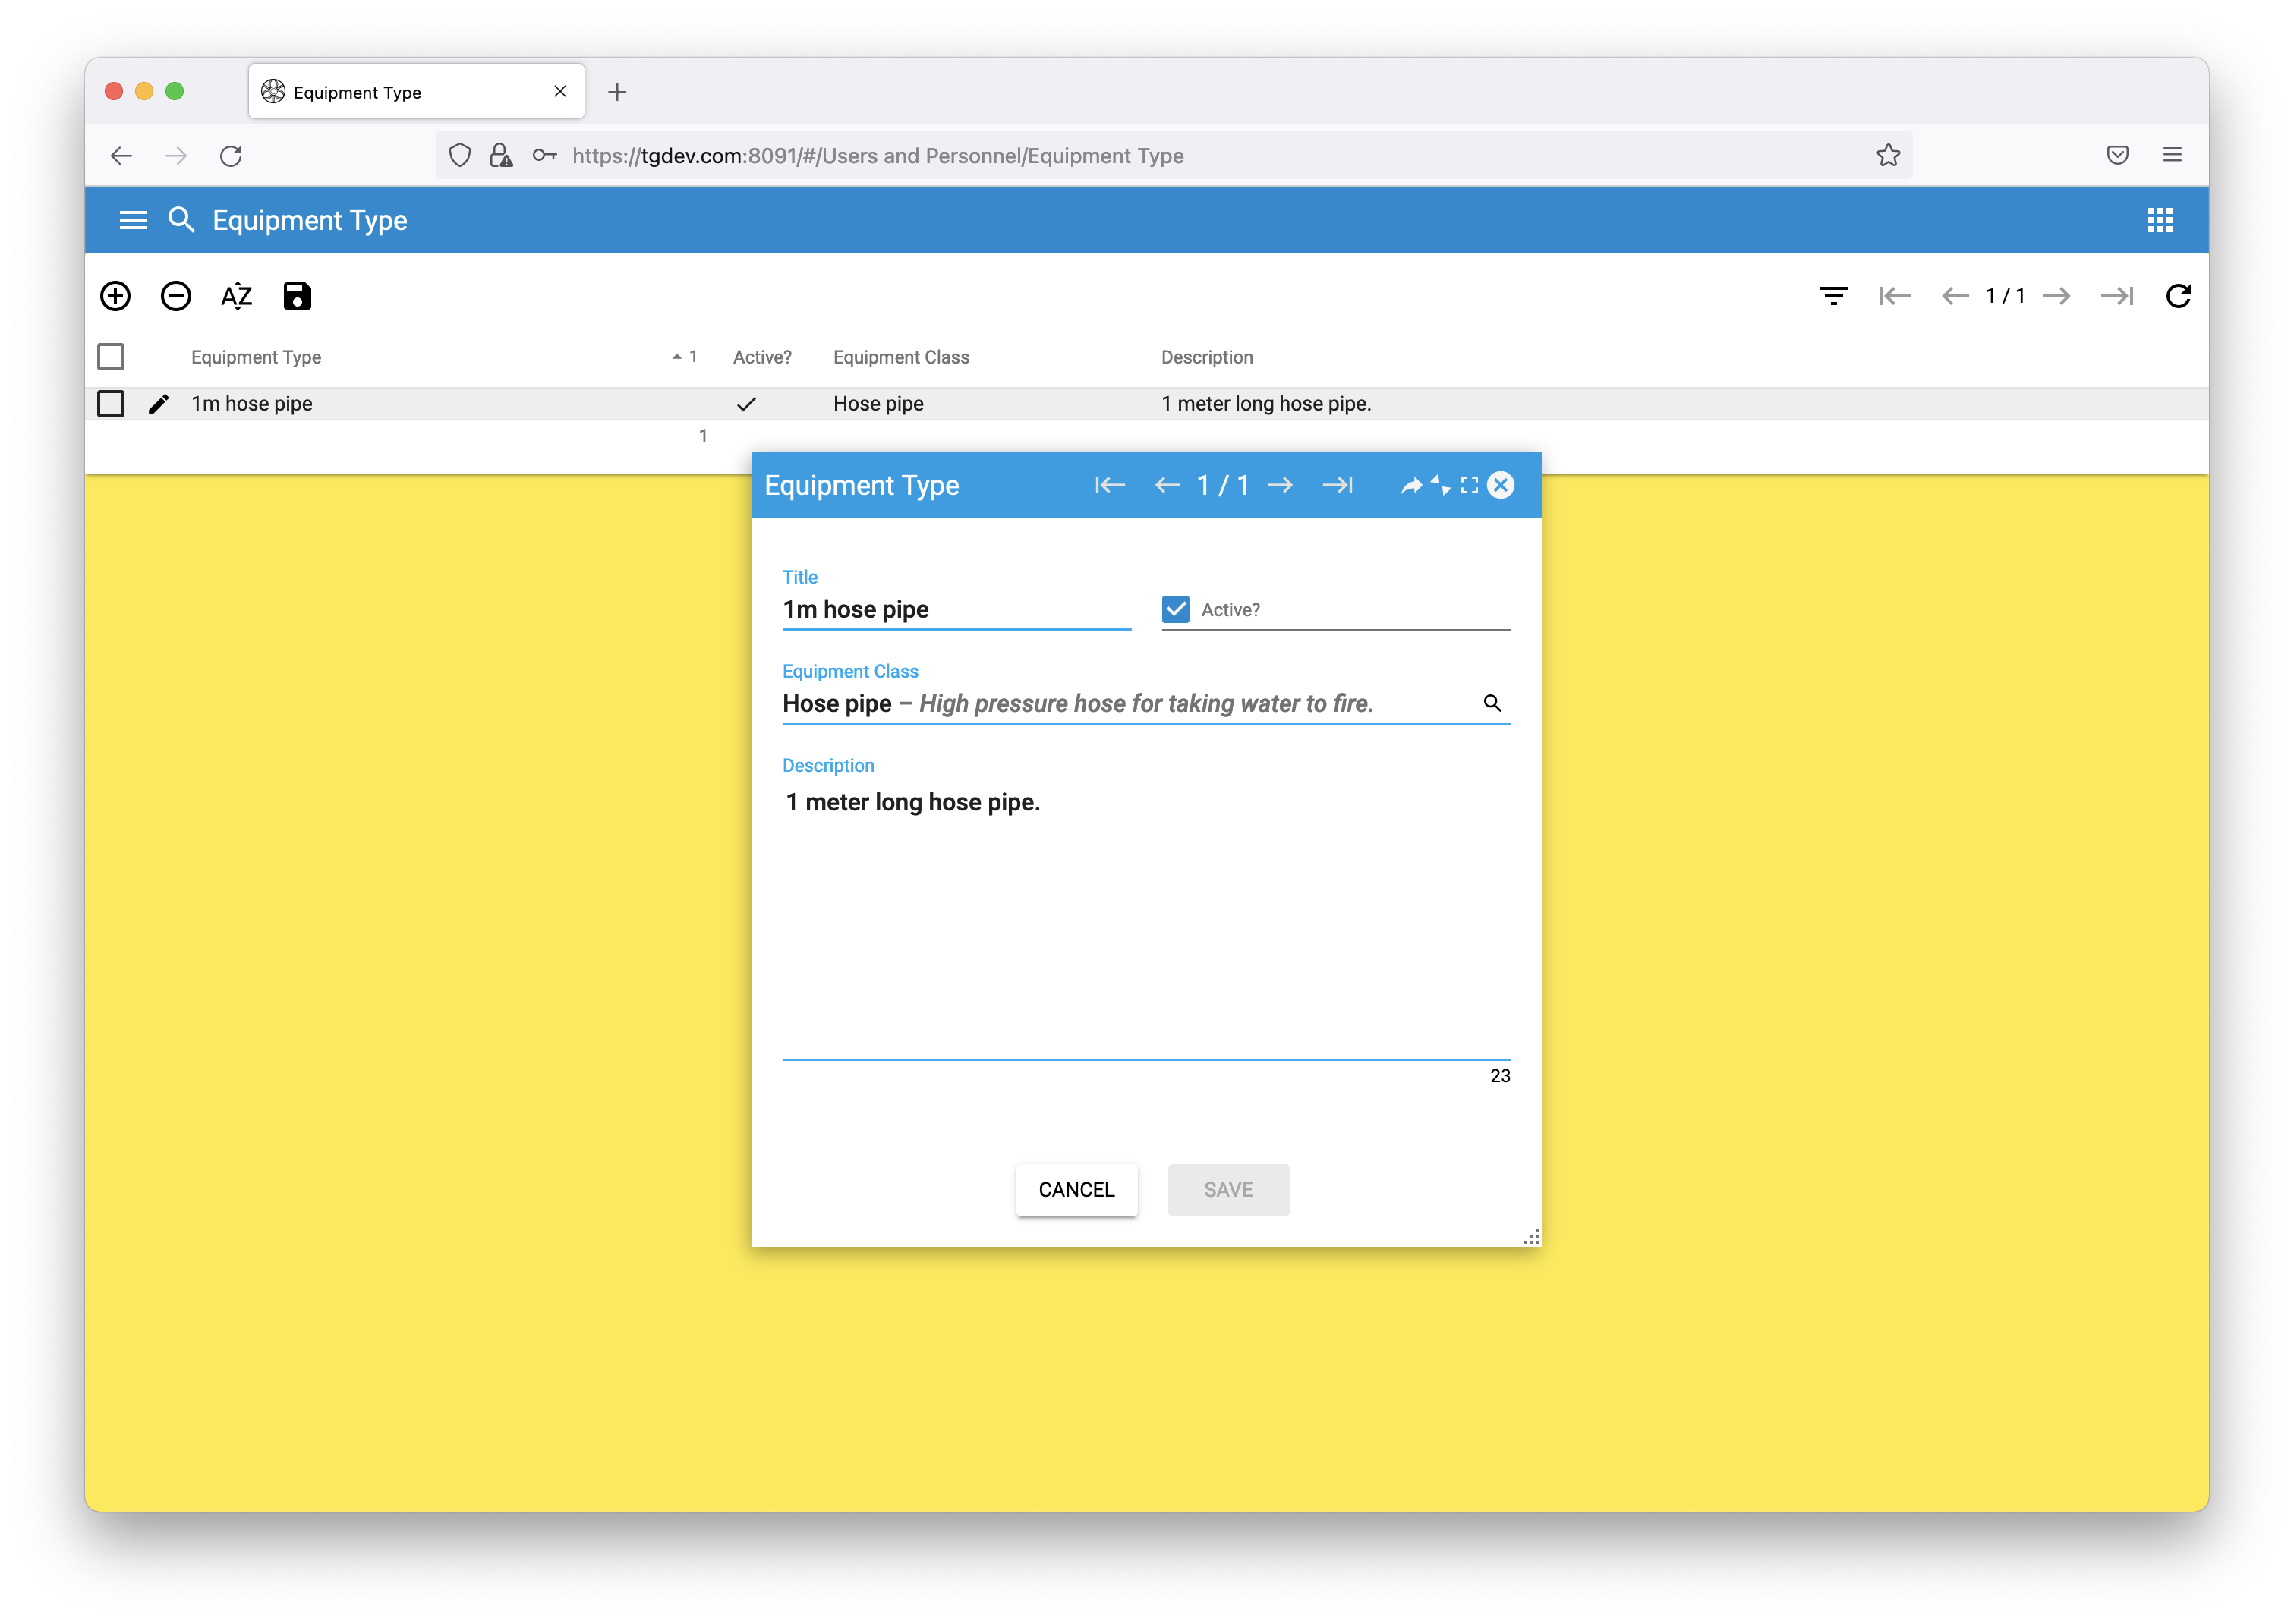
\includegraphics[width=0.95\linewidth]{sections/equipment/images/Fig.11.png}
	\caption{Equipment type editing.}\label{sections/equipment/images/Fig.11}
	\end{figure}
	
\newpage	
\subsection{Equipment}

In order to perform registration, classification and tracking of equipment correctly, users can create equipment. Possible equipment are pipe, lightning, etc. When creating a new equipment, users have to fill in its title without white spaces, activity status, equipment type and vehicle it belongs to, which are auto-completed, and its description, as displayed on \hyperref[sections/equipment/images/Fig.12]{Fig.~\ref*{sections/equipment/images/Fig.12}}. The number of equipment is auto-generated in chronological order after it was saved. 

    \begin{figure}[!htbp]
	\centering
	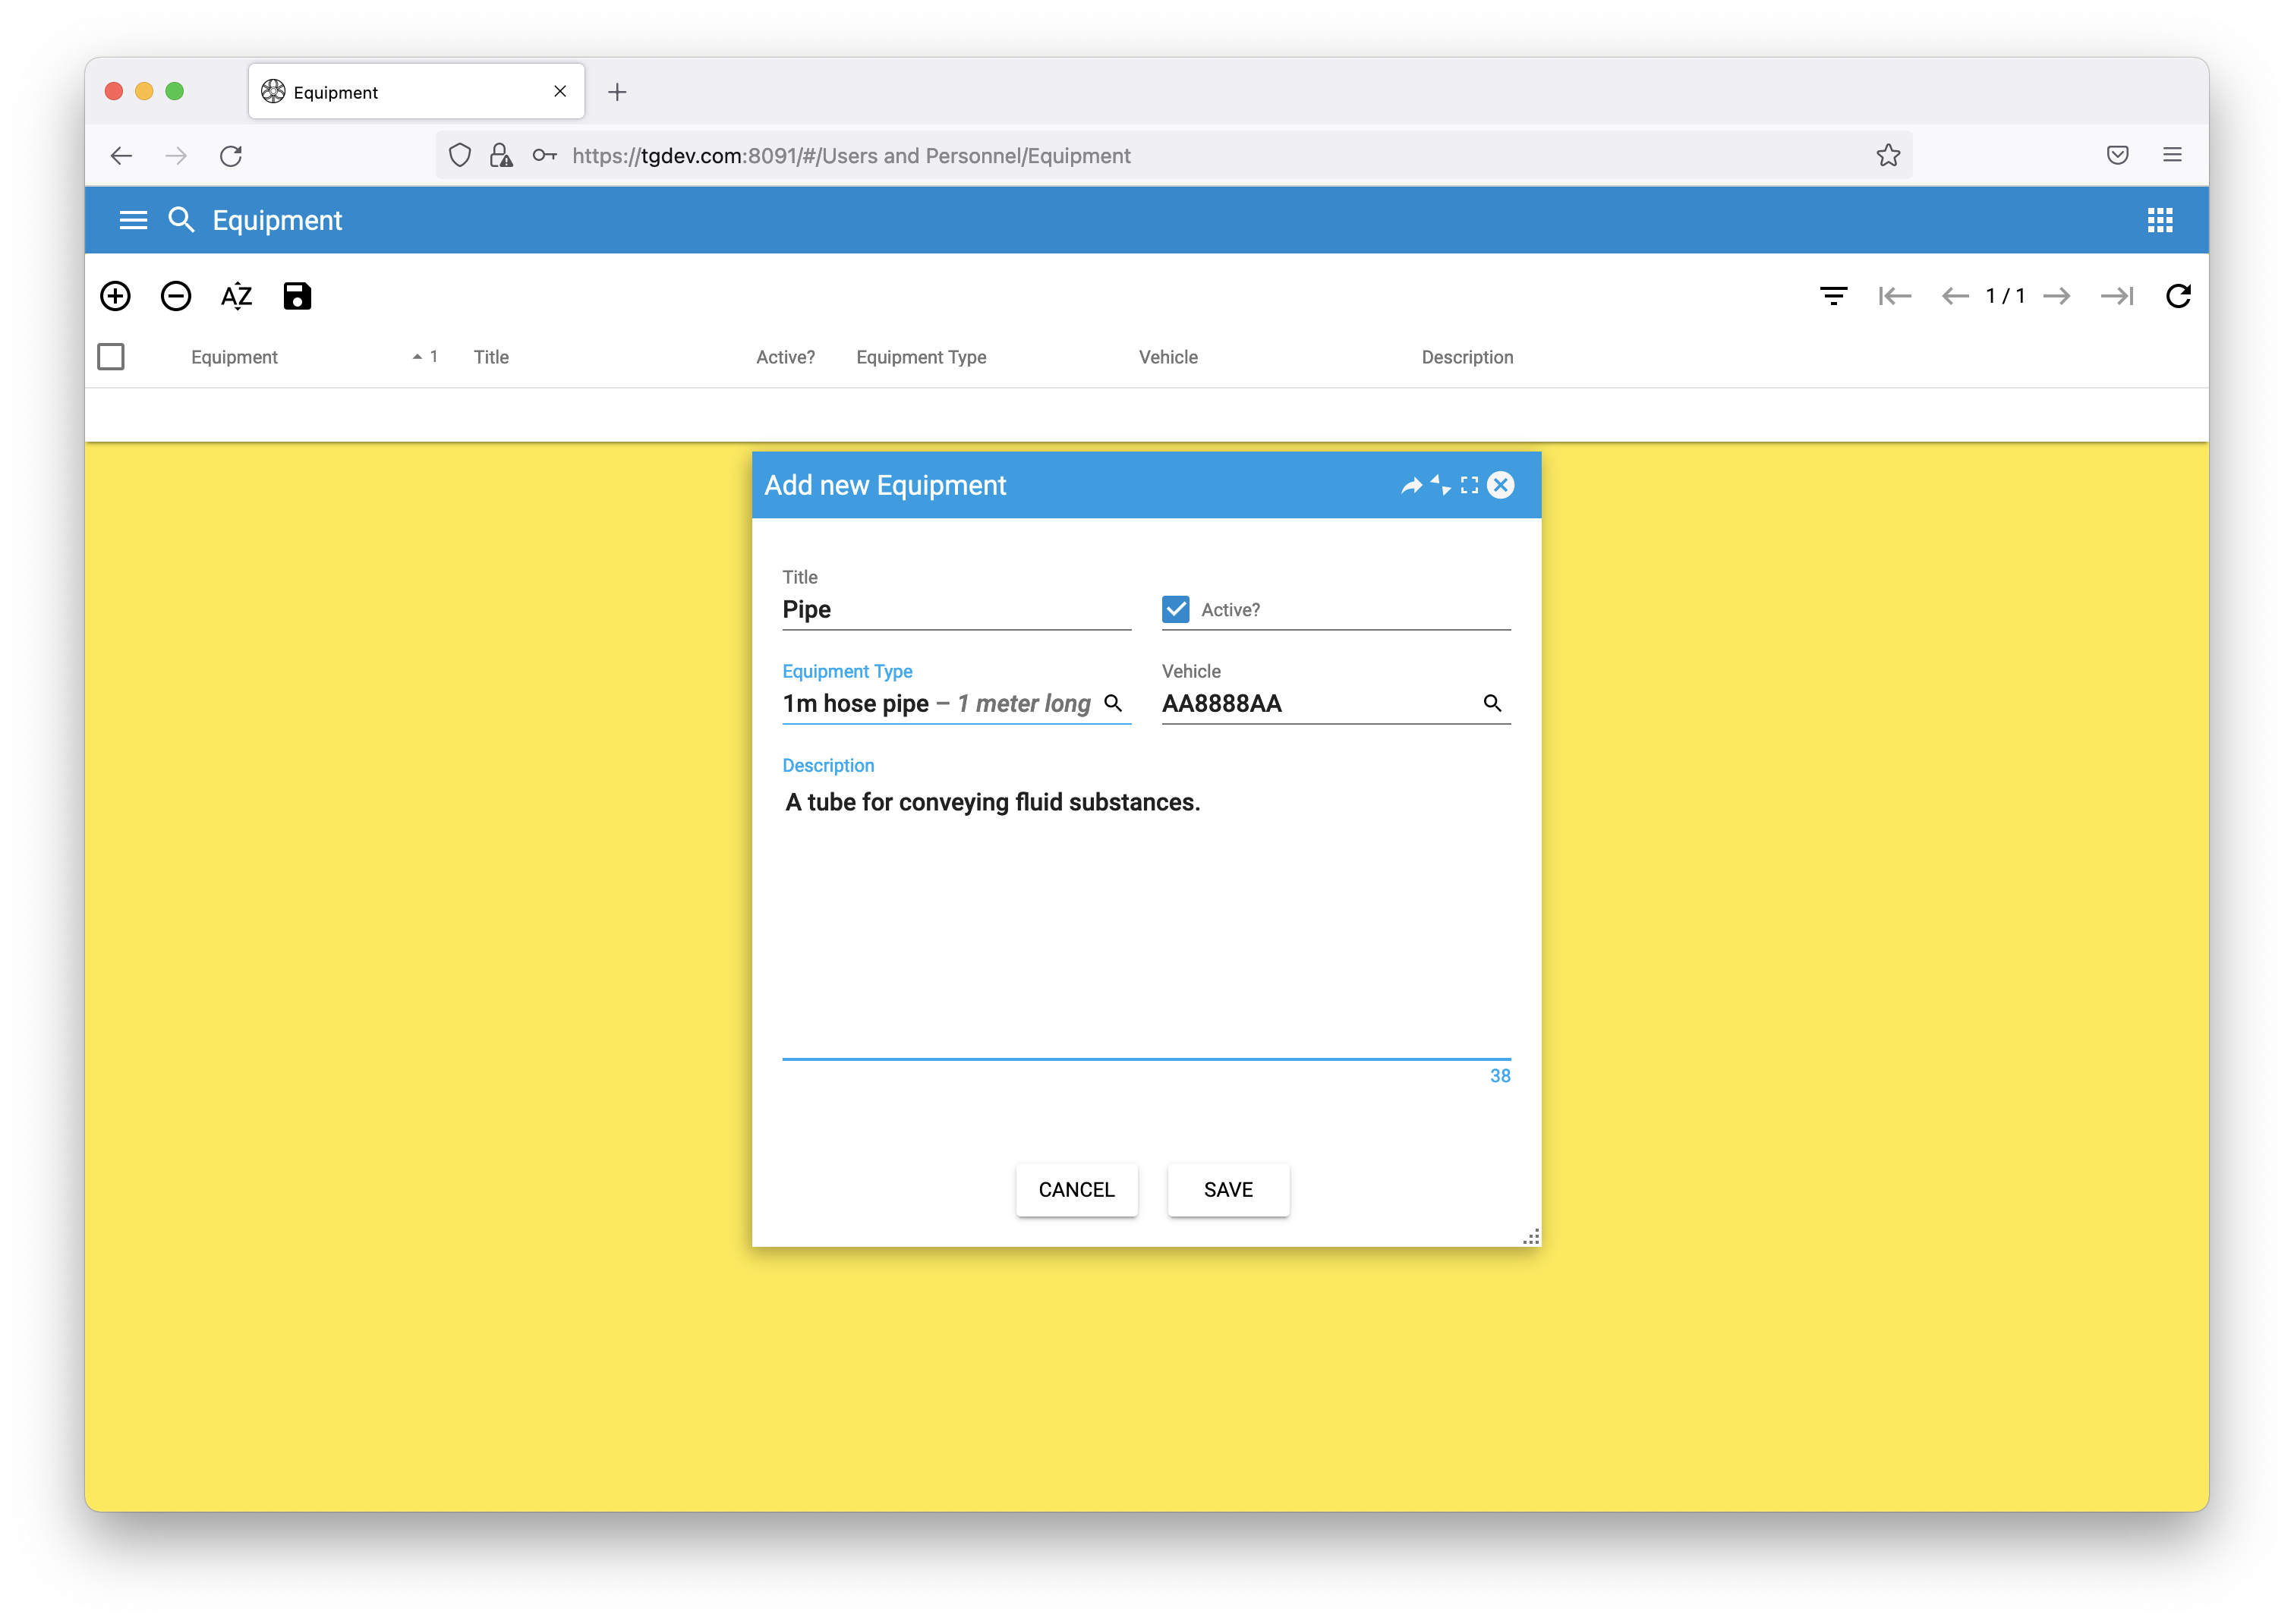
\includegraphics[width=0.95\linewidth]{sections/equipment/images/Fig.12.png}
	\caption{Equipment creation.}\label{sections/equipment/images/Fig.12}
	\end{figure}

\newpage
Users can search for existing equipment either by specifying number, which is auto-completed, activity status, title, equipment type and vehicle they belong to and which are auto-completed, or all, as displayed on \hyperref[sections/equipment/images/Fig.13]{Fig.~\ref*{sections/equipment/images/Fig.13}}.

    \begin{figure}[!htbp]
	\centering
	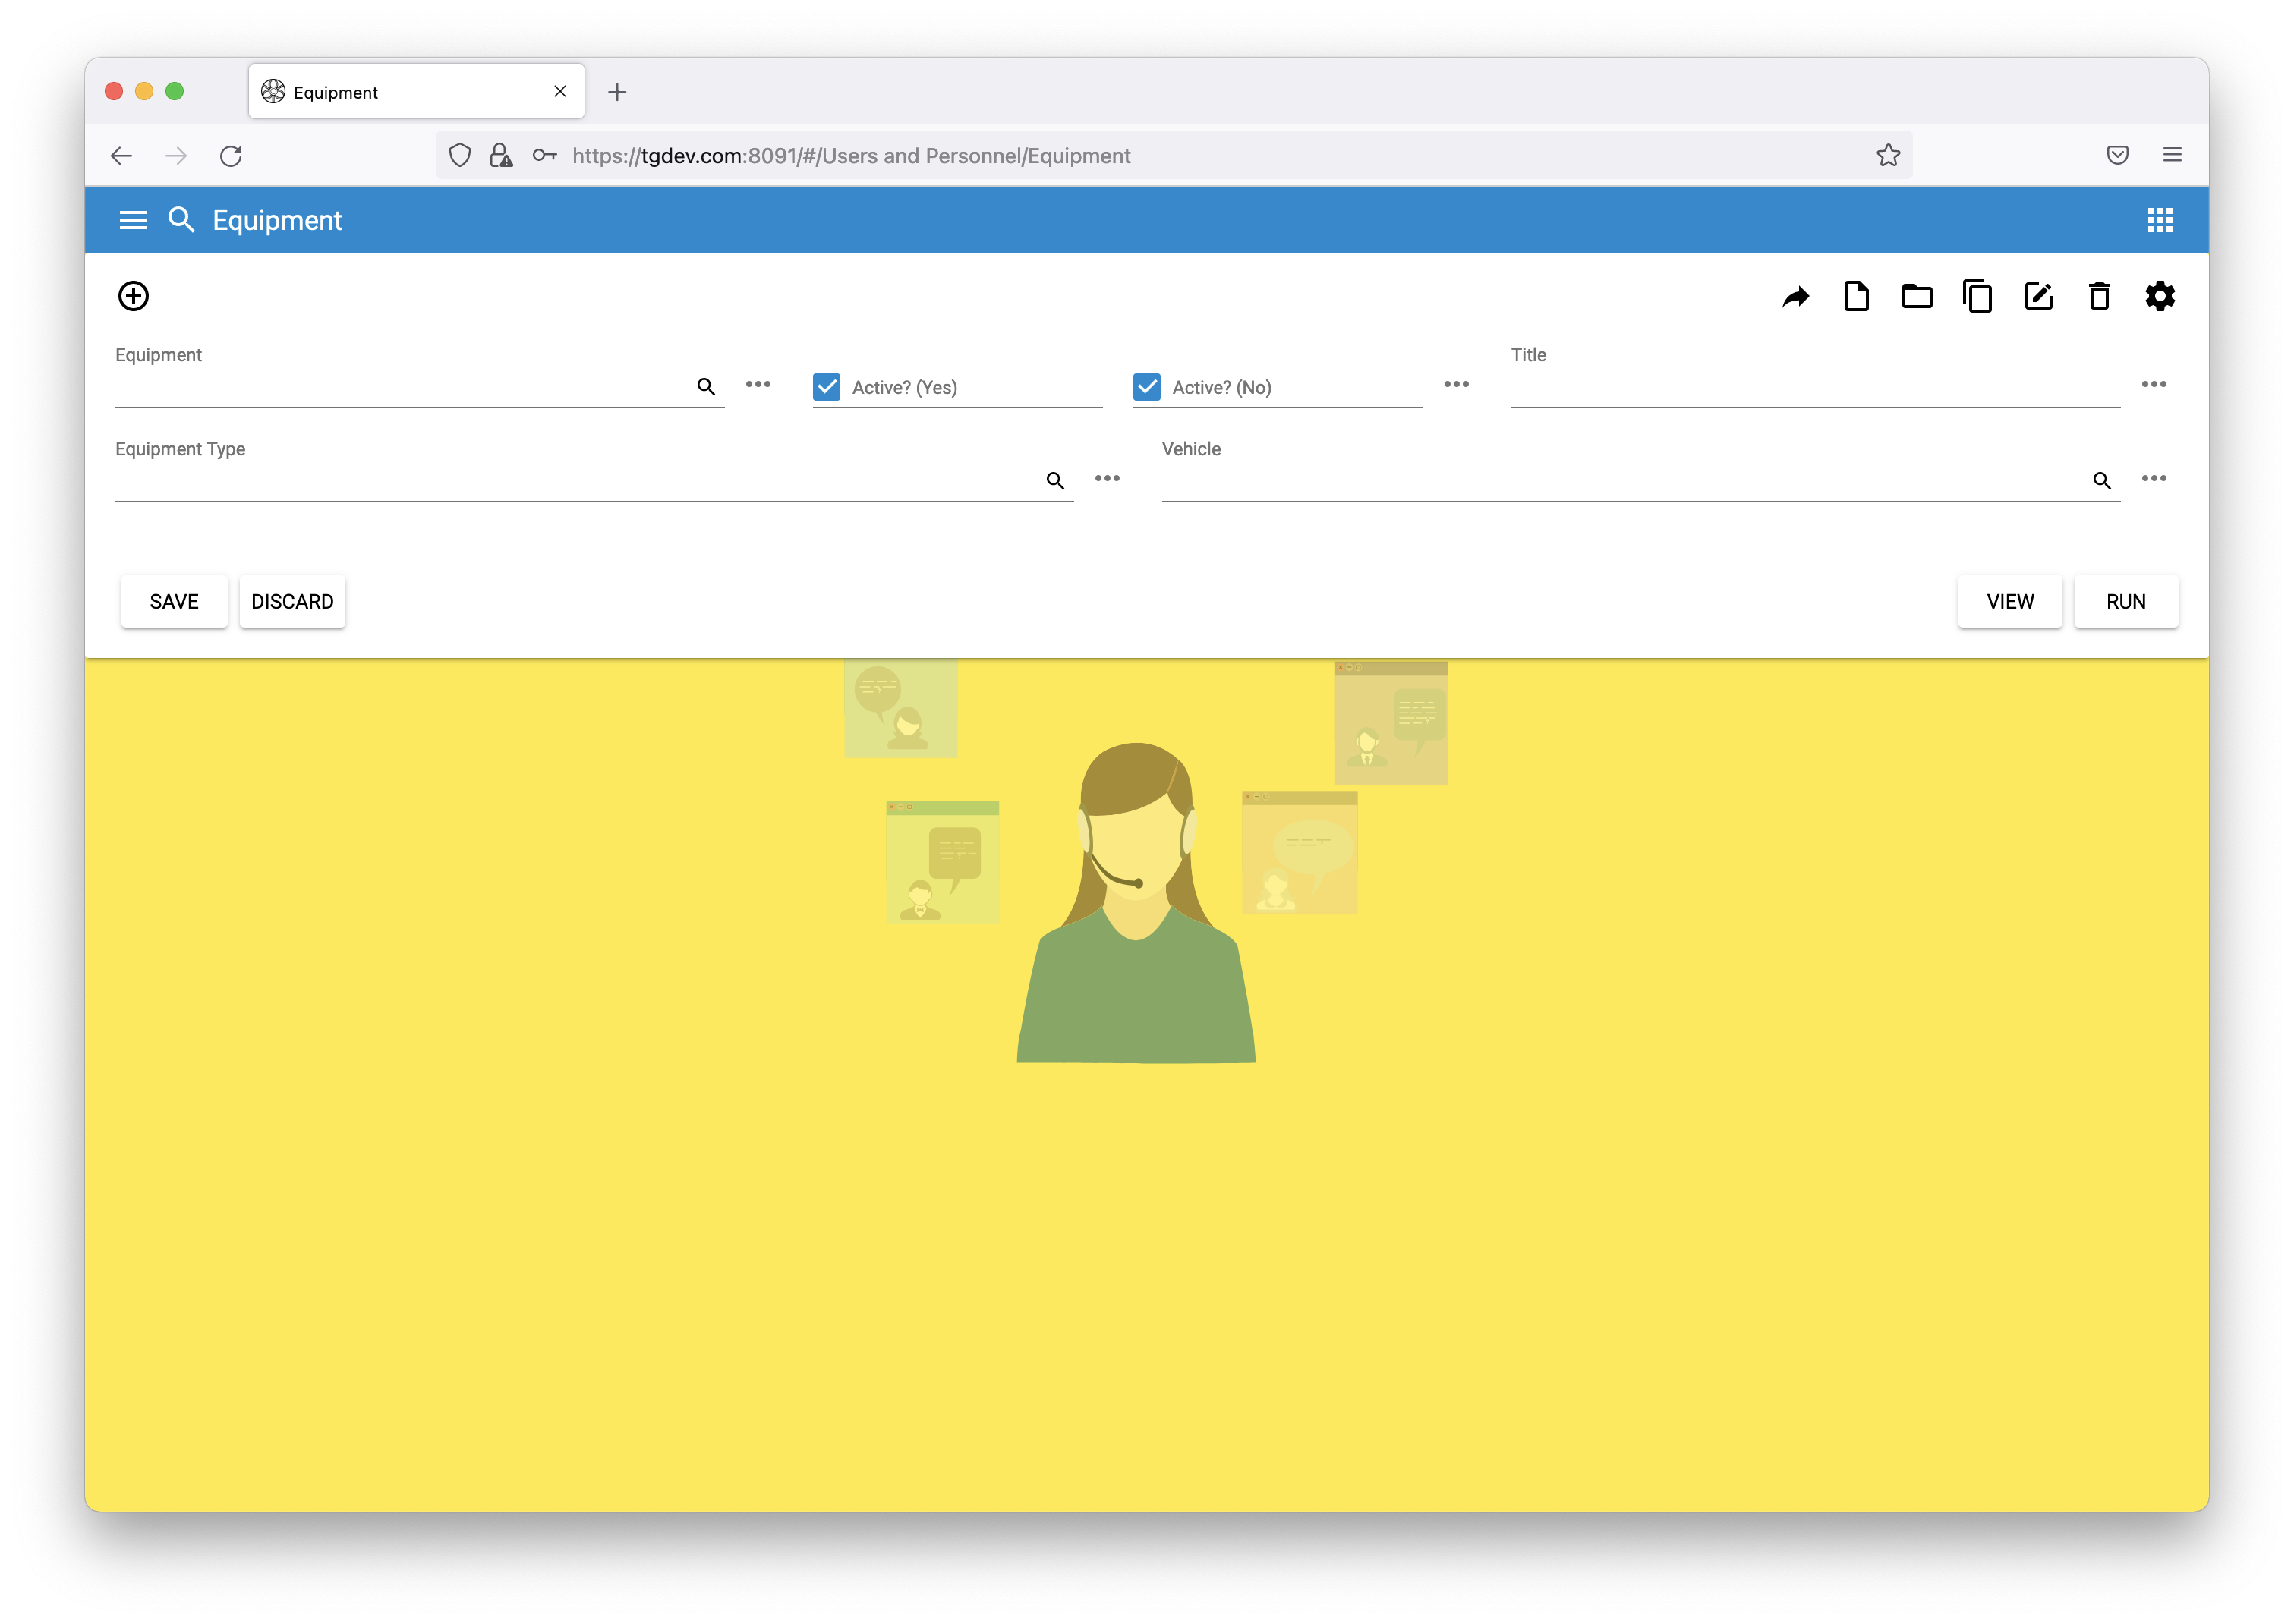
\includegraphics[width=0.95\linewidth]{sections/equipment/images/Fig.13.png}
	\caption{Equipment search query.}\label{sections/equipment/images/Fig.13}
	\end{figure}
	
\newpage
Search results are displayed along with number, title, activity status, equipment type, vehicle and description of the relevant equipment, as displayed on \hyperref[sections/equipment/images/Fig.14]{Fig.~\ref*{sections/equipment/images/Fig.14}}.

    \begin{figure}[!htbp]
	\centering
	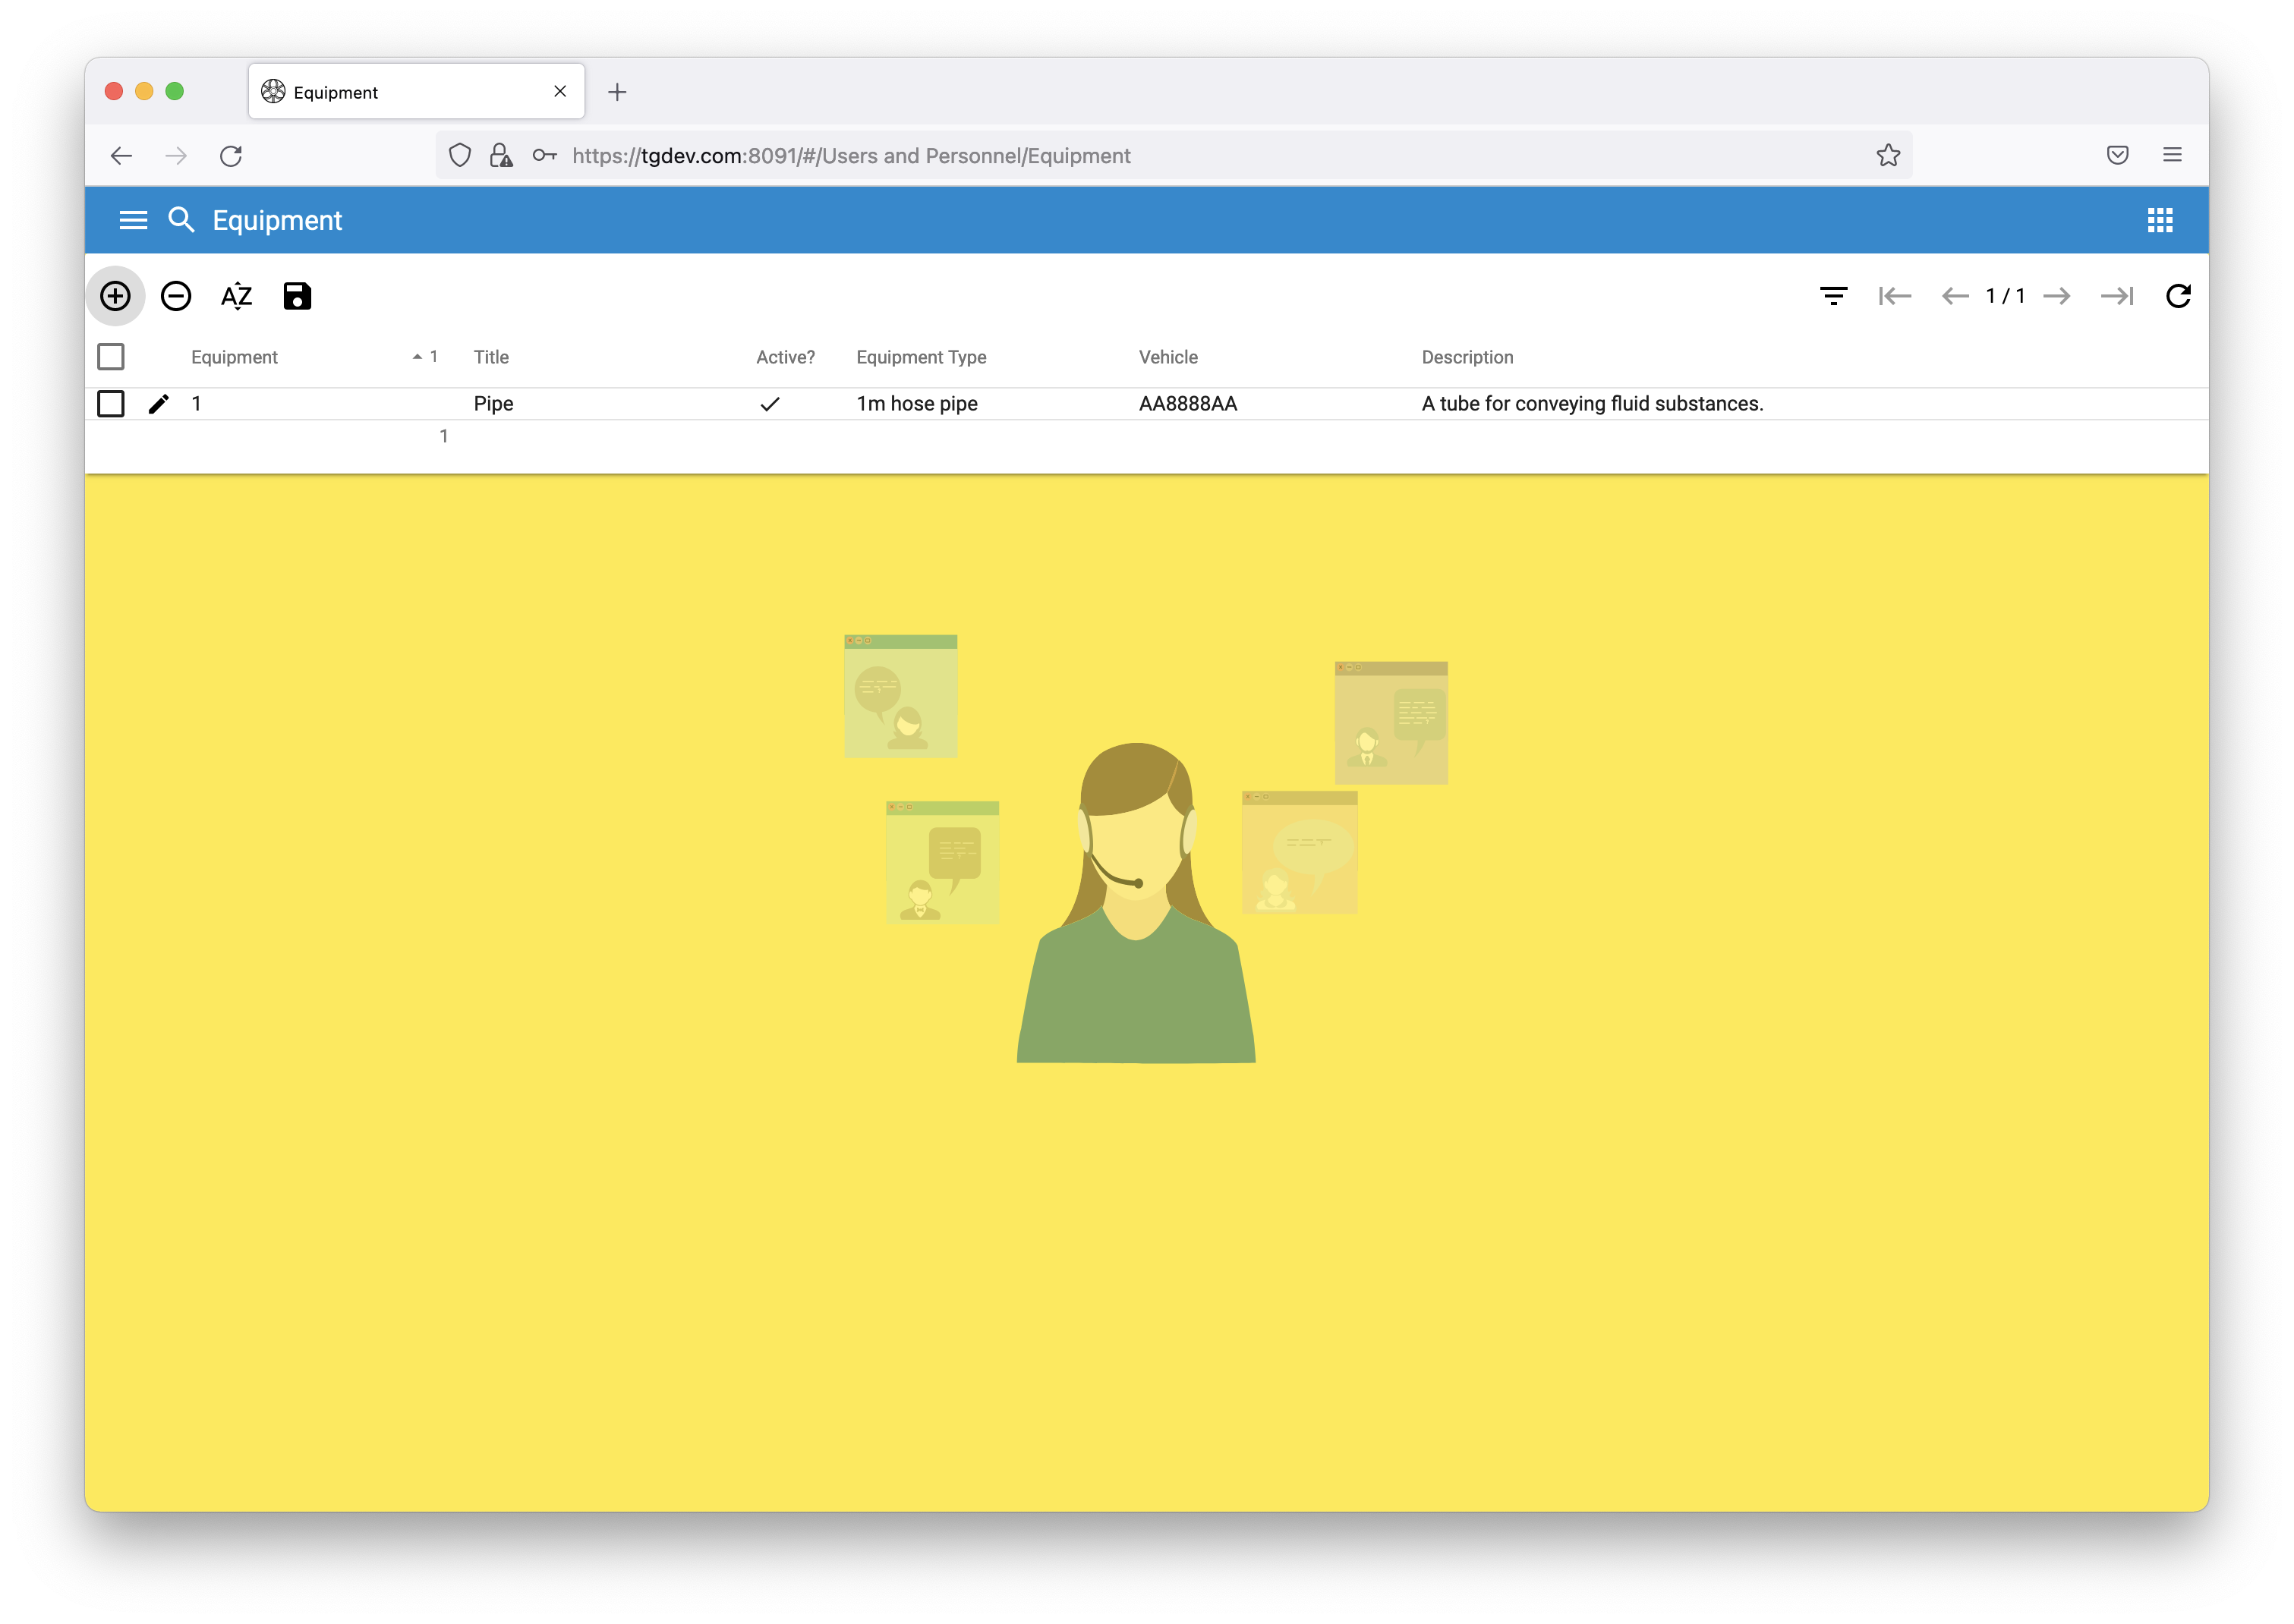
\includegraphics[width=0.95\linewidth]{sections/equipment/images/Fig.14.png}
	\caption{Equipment search results.}\label{sections/equipment/images/Fig.14}
	\end{figure}

\newpage
Users can edit existing equipment. As displayed on \hyperref[sections/equipment/images/Fig.15]{Fig.~\ref*{sections/equipment/images/Fig.15}}, users can edit title, activity status, equipment type, vehicle and description of the specific equipment.

    \begin{figure}[!htbp]
	\centering
	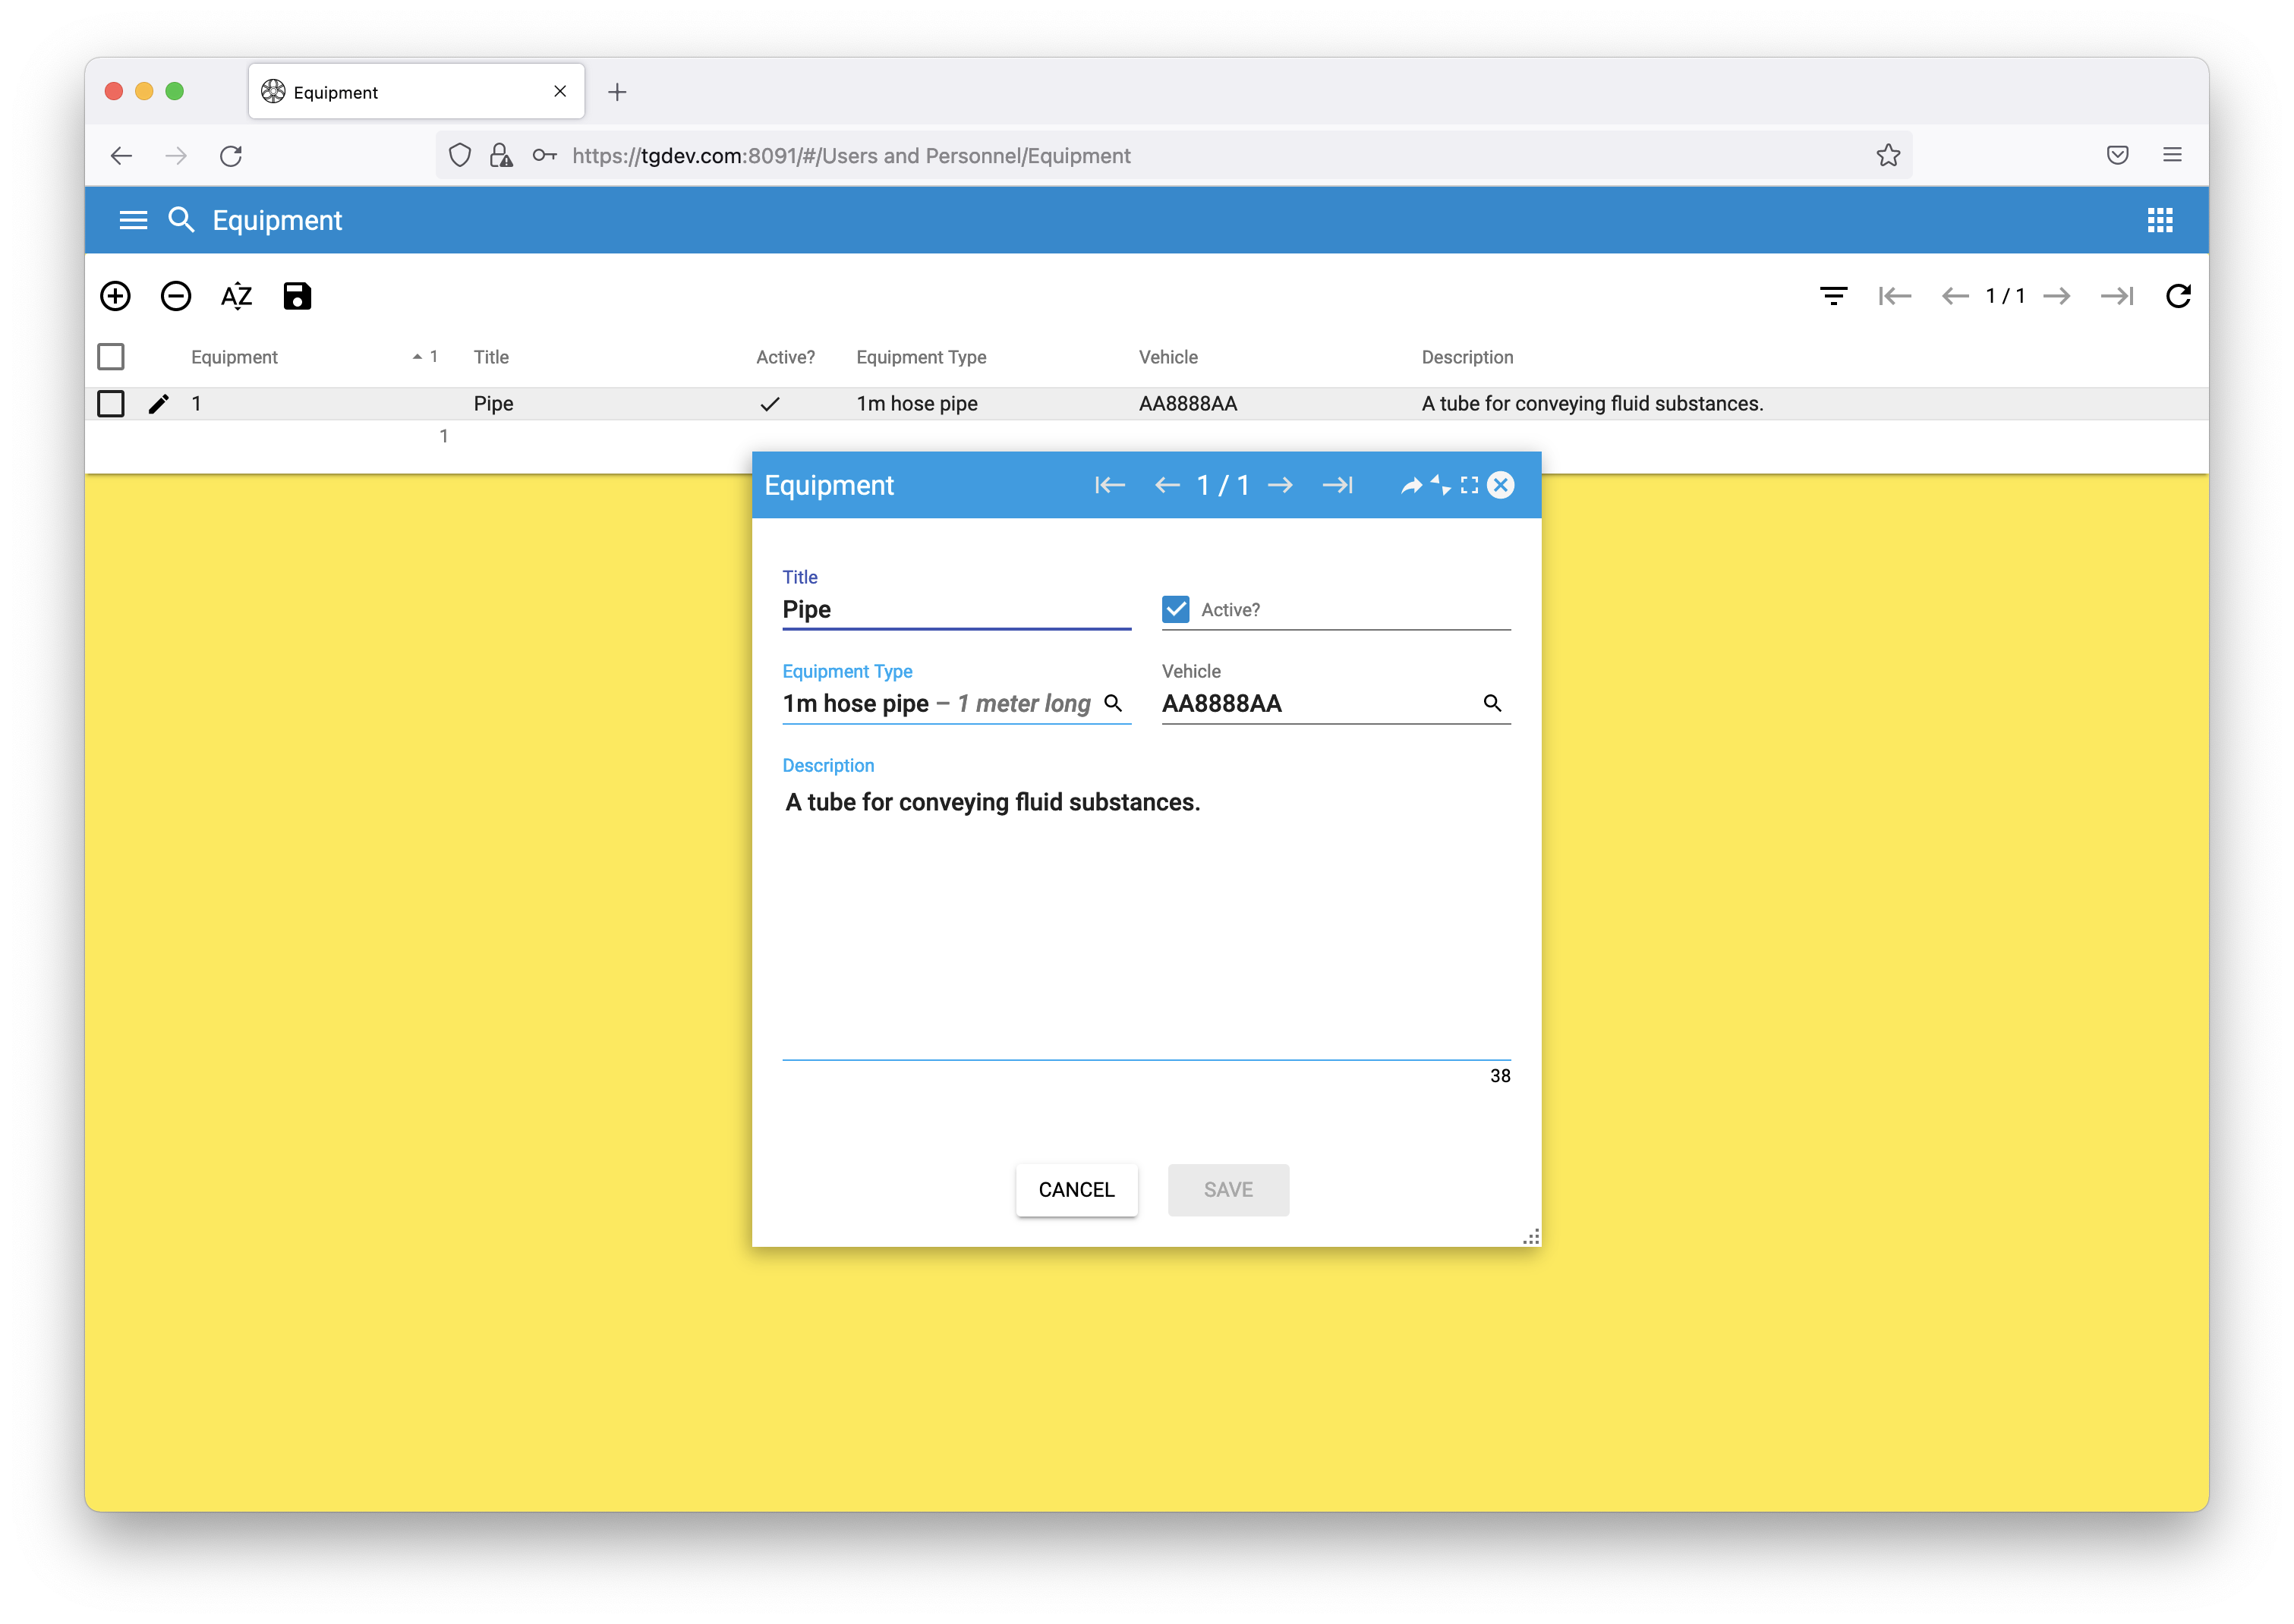
\includegraphics[width=0.95\linewidth]{sections/equipment/images/Fig.15.png}
	\caption{Equipment editing.}\label{sections/equipment/images/Fig.15}
	\end{figure}